\documentclass[12pt,a4paper]{article}
\usepackage[american]{babel}
\usepackage{amsmath}
\usepackage{amsfonts}
\usepackage{amssymb}
\usepackage[utf8x]{inputenc}
\setlength{\parindent}{1.5em}
\setlength{\parskip}{0.5em}
\usepackage{indentfirst}
\usepackage{float}
\usepackage{systeme}
\usepackage[bitstream-charter]{mathdesign} %% option 'sfdefault' activates Fira Sans as the default text font
\usepackage[T1]{fontenc}
% \usepackage[frenchmath]{newtxmath}
\usepackage[frenchmath]{mathastext}
% \renewcommand*\oldstylenums[1]{{\firaoldstyle #1}}
\usepackage[titles]{tocloft}
\renewcommand{\cftdot}{}
\usepackage[colorlinks=true, allcolors=magenta, backref=page]{hyperref}
\usepackage{url}
\usepackage{graphicx}

% Colors
\usepackage[dvipsnames]{xcolor}
\definecolor{fireopal}{rgb}{0.93, 0.38, 0.33}
\definecolor{aquamarine}{rgb}{0.38, 0.83, 0.58}
\definecolor{mintgreen}{rgb}{0.67, 0.97, 0.51}
\definecolor{crayola}{rgb}{1, 0.85, 0.49}
\definecolor{tangerine}{rgb}{1, 0.61, 0.52}

\usepackage{amsthm}
\newtheoremstyle{break}%
{}{}%
{\itshape}{}%
{\bfseries}{}% % Note that final punctuation is omitted.
{\newline}{}
%\theoremstyle{break}
\theoremstyle{definition}
\newtheorem{theorem}{Theorem}[section]
\newtheorem{corollary}[theorem]{Corollary}
\newtheorem{lemma}[theorem]{Lemma}
\newtheorem{remark}[theorem]{Remark}
\newtheorem{proposition}[theorem]{Proposition}
\newtheorem{example}{Example}[section]
\newtheorem{definition}{Definition}[section]
\renewcommand\qedsymbol{$\blacksquare$}

% TColorBox
%\usepackage{tcolorbox}
%\tcbuselibrary{theorems,breakable}
%\tcbsetforeverylayer{autoparskip, breakable}
%\newtcbtheorem[number within=section]{thm}{Theorem}%
%{colback=white!5,colframe=fireopal!35!black,fonttitle=\bfseries, arc=0mm}{theorem}
%\newtcbtheorem[number within=section]{corollary}{Corollary}%
%{colback=white!5,colframe=aquamarine!35!black,fonttitle=\bfseries, arc=0mm}{theorem}
%\newtcbtheorem[number within=section]{example}{Example}%
%{colback=white!5,colframe=tangerine!35!black,fonttitle=\bfseries, arc=0mm}{theorem}
%\newtcbtheorem[number within=section]{defn}{Definition}%
%{colback=white!5,colframe=mintgreen!35!black,fonttitle=\bfseries, arc=0mm}{theorem}

% NEW COMMANDS
\newcommand\restr[2]{{% we make the whole thing an ordinary symbol
  \left.\kern-\nulldelimiterspace % automatically resize the bar with \right
  #1 % the function
  \vphantom{\big|} % pretend it's a little taller at normal size
  \right|_{#2} % this is the delimiter
  }}

\usepackage{quiver}

%\usepackage{sectsty}
%\subsectionfont{\color{RubineRed}}
\hypersetup{
    colorlinks=true,
    linkcolor=fireopal,
    filecolor=aquamarine,      
    urlcolor=fireopal,
    pdftitle={Analysis: Study Notes},
    pdfpagemode=FitH,
}
\author{\href{https://github.com/adairneto}{Adair Antonio da Silva Neto}}
\title{Analysis: Study Notes}

\begin{document}

\clearpage\maketitle
\thispagestyle{empty}

\newpage

\tableofcontents

\newpage
\clearpage
\setcounter{page}{1}

\section{Finite and Infinite Sets}

\subsection{Basic Definitions}

The `vocabulary' needed for Analysis comes from set theory. So, before going further, what is a set?

Intuitively, a \textbf{set} is any collection of objects, called \textbf{elements} of the set.

\begin{definition}
	Some basic notation:
	\begin{enumerate}
		\item $x \in A$ means that $x$ is an element of $A$. If $x$ is not an element of $A$, we write $x \notin A$.
		\item The \textbf{union} of two sets $A$ and $B$ is denoted by $A \cup B$ and is defined by \[ x \in A \cup B \iff x \in A \text{ or } x \in B \]
		\item The \textbf{intersection} $A \cap B$ is the set defined by \[ x \in A \cap B \iff x \in A \text{ and } x \in B \] If the intersection $A \cap B$ is the empty set $\emptyset$, then these sets are said to be \textbf{disjoint}.
		\item The \textbf{inclusion} $A \subseteq B$ means that every element of $A$ is also an element of $B$. And we say that $A$ is a \textbf{subset} of $B$, or $B$ \textbf{contains} $A$. If there is some element in $B$ which is not in $A$, then $A$ is said to be a \textbf{proper subset} of $B$, denoted by $A \subsetneq B$. To say that $A = B$ means that $A \subseteq B$ and $B \subseteq A$, i.e., both sets have exactly the same elements.
		\item Given $A \subseteq \textbf{R}$, the \textbf{complement} of $A$, denoted by $A^c$ is the set of all elements in $\textbf{R}$ which are not in $A$. \[ A^c = \{ x \in \textbf{R} : x \notin A \} \]
	\end{enumerate}
\end{definition}

Analysis is concerned mainly about the construction of Real Numbers and functions between them. The concept of function also comes from set theory. Here, we'll define it and introduce some basic nomenclature to help our discussions.

\begin{definition}[Function]
	A \textbf{function} from a set $A$ into a set $B$ is a rule or mapping that associates each element $x \in A$ to a single element of $B$, denoted by $f : A \longrightarrow B$. And the expression $f(x)$ represents the element of $B$ associated with $x$ by $f$.
	
	The set $A$ is called \textbf{domain of $f$}, and the elements $f(x)$ are called the \textbf{values of $f$}. The set of all values of $f$ is called \textbf{range of $f$}.
\end{definition}

\begin{definition}[Surjection]
	Let $f$ be a function of $A$ into $B$. If $E \subseteq A$, then $f(E)$ is the set of all elements $f(x)$ such that $x \in E$ and we call $f(E)$ the \textbf{image} of $E$ under $f$. Clearly, $f(A) \subseteq B$. If $f(A) = B$, then $f$ maps $A$ \textbf{onto} $B$ and is called a \textbf{surjective function}. In other words, for all $y \in B$ there is at least one $x \in A$ such that $f(x) = y$.
\end{definition}

\begin{definition}[Inverse image]
	If $C \subseteq B$, then $f^{-1}(C)$ denotes the set of all $x \in A$ such that $f(x) \in C$, and is called \textbf{inverse image of $C$ under $f$} or \textbf{pre-image}.
	If $y \in B$, then $f^{-1}(y)$ is the set of all $x \in A$ such that $f(x) = y$.
	\[ f^{-1}(C) = \{ a \in A : f(a) \in C \} \]
\end{definition}

\begin{definition}[Injection]
	If, for each $y \in B$, $f^{-1}(y)$ consist of at most one element of $A$, then $f$ is said to be a \textbf{one-to-one} mapping of $A$ into $B$, also called a \textbf{injective function}. I.e., $f(x_1) \neq f(x_2)$ whenever $x_1 \neq x_2$.
\end{definition}

\begin{definition}[Bijection]
	If there exists a one-to-one mapping of $A$ onto $B$ (i.e. an injective and surjective function), then we can say that $A$ and $B$ can be put in \textbf{one-to-one correspondence}, or that $A$ and $B$ have the same \textbf{cardinal number}, and the function satisfying this property is called a \textbf{bijective function}, and we write $A \sim B$. This relation is an \textbf{equivalence relation}.
\end{definition}

\begin{definition}[Left inverse]
	Given $f : A \longrightarrow B$ and $g : B \longrightarrow A$, we say that $g$ is a \textbf{left inverse} of $f$ when $g \circ f = \text{id}_A$.
\end{definition}

\begin{proposition}\label{propleftinv}
	A function $f : A \longrightarrow B$ has a left inverse iff. it is injective.
\end{proposition}

\begin{definition}[Right inverse]
	Given $f : A \longrightarrow B$ and $g : B \longrightarrow A$, we say that $g$ is a \textbf{right inverse} of $f$ when $f \circ g = \text{id}_B$.
\end{definition}

\begin{proposition}\label{proprightinv}
	A function $f : A \longrightarrow B$ has a right inverse iff. it is surjective.
\end{proposition}

\begin{definition}[Inverse function]
	A function $g : B \longrightarrow A$ is said to be an \textbf{inverse} of $f : A \longrightarrow B$ when $g$ is both a left and a right inverse of $f$.
\end{definition}

\begin{proposition}
	A function $f$ has an inverse function iff. it is a bijection.
\end{proposition}

\begin{proof}
	Follows from Proposition \ref{propleftinv} and Proposition \ref{proprightinv}.
\end{proof}

\begin{proposition}
	If a function $f : A \longrightarrow B$ has an inverse, then the inverse is unique.
\end{proposition}

\begin{proof}
	Suppose that $g : B \longleftrightarrow A$ and $h : B \longleftrightarrow A$ are both inverses of $f$. Then
	\[ h = h \circ \text{id}_B = h \circ (f \circ g) = (h \circ f) \circ g = \text{id}_A \circ g = g \]
	That means that if $f$ has a left inverse $h$ and a right inverse $g$, then $h = g$ and $f$ has an inverse.
\end{proof}

\begin{corollary}
	If $f : A \longrightarrow B$ and $g : B \longrightarrow C$ are bijections, then \[ (g \circ f)^{-1} = f^{-1} \circ g^{-1} \]
\end{corollary}

\subsection{Natural numbers}

The set of natural numbers, denoted by $\textbf{N}$, is defined by the following axioms, known as \textbf{Peano Axioms}.

\begin{enumerate}
	\item[A1] There is an injective function $s : \textbf{N} \longrightarrow \textbf{N}$ such that the image $s(n)$ is called the \textbf{successor} of $n$.
	\item[A2] There is a unique number $1 \in \textbf{N}$ such that $1 \neq s(n)$ for all $n \in \textbf{N}$. I.e., $1$ is not the successor of any natural number.
	\item[A3] If $X \subseteq \textbf{N}$ is such that $1 \in X$ and $s(X) \subseteq X$, then $X = \textbf{N}$. This axiom is known as the \textbf{Principle of mathematical induction}.
\end{enumerate}

We will denote $2 = s(1), 3 = s(2) = s(s(1)), \ldots, n = s^{n-1}(1) = \underbrace{s \circ s \circ \ldots \circ s}_{(n-1) \text{ times}}(1)$.

\begin{definition}[Addition]
	The \textbf{addition} in $\textbf{N}$ is defined by the function
	\begin{equation*}
		\begin{aligned}
			\textbf{N} \times \textbf{N} & \longrightarrow \textbf{N} \\
			(m,n) & \mapsto	m+n
		\end{aligned}
	\end{equation*}
	satisfying the following properties:
	\begin{enumerate}
		\item $m+1 = s(m)$.
		\item $m+s(n) = s(m+n)$.
	\end{enumerate}
\end{definition}

\begin{theorem}
	For all $m,n,p \in \textbf{N}$:
	\begin{itemize}
		\item $(m+n)+p = m+(n+p)$.
		\item $m+n = n+m$.
		\item If $m+p = n+p$, then $m = n$.
	\end{itemize}
\end{theorem}

\begin{definition}[Multiplication]
	The \textbf{multiplication} is defined by the function
		\begin{equation*}
		\begin{aligned}
			\textbf{N} \times \textbf{N} & \longrightarrow \textbf{N} \\
			(m,n) & \mapsto	m \cdot n
		\end{aligned}
	\end{equation*}
	satisfying:
	\begin{enumerate}
		\item $m \cdot 1 = m$.
		\item $m \cdot s(n) = m \cdot n + m$.
	\end{enumerate}
\end{definition}

And we will simply denote $m \cdot n$ by $mn$.

\begin{theorem}
	For all $m,n,p \in \textbf{N}$,
	\begin{itemize}
		\item $p(m+n) = pm+pn$.
		\item $(m+n)p = mp+np$.
		\item $(mn)p = m(np)$.
		\item $mn = nm$.
		\item If $mp=np$, then $m=n$.
	\end{itemize}
\end{theorem}

Given two natural numbers $m,n$ we write $m < n$ if there is a natural number $p$ such that $n = m+p$. Naturally,

\begin{theorem} \hfill
	\begin{itemize}
		\item If $m<n$ and $n<p$, then $m<p$.
		\item (Trichotomy law) One and only one of the following is true: $m = n$, or $m < n$, or $m>n$.
	\end{itemize}
\end{theorem}

This idea of order between natural numbers motivates the following theorem.

\begin{theorem}[Well ordering principle]
	Every non-empty subset $A \subseteq \textbf{N}$ has a minimum element. I.e., there is an element $n \in A$ such that $n \leq m$ for all $m \in A$.
\end{theorem}

\begin{proof}
	If $1 \in A$, then $1 \leq k$ for all $k \in A$.
	
	Assume $1 \notin A$ and define $J_m = \textbf{N} \setminus \{1,2,\ldots, m\}$ for every $m \in \textbf{N}$.
	
	Consider the following set $B = \{ m \in \textbf{N} : A \subseteq J_m \}$. Since $1 \notin A$, it follows that $A \subseteq J_1$. Hence, $1 \in B$. 
	
	Given that $A$ is non-empty, there is an element $m \in A$. And since $m \notin J_m$, we have $A \not\subset J_m$. Hence, $m \notin B$, which implies that $B \neq \textbf{N}$. 
	
	Finally, since $1 \in B$ and $B \neq \textbf{N}$, there is $n \in B$ such that $n+1 \notin B$ by the induction principle. Therefore, $A \not\subset J_{n+1}$, and hence $n+1 \leq k$, for all $k \in A$.
\end{proof}

\subsection{Finite and Infinite sets}

The following two lemmas will allow us to distinguish between finite and infinite sets.

\begin{lemma}\label{two-bij-fun}
	Let $f:A \longrightarrow B$ be a bijective function. Given $a \in A$ and $b \in B$, there is always a bijective function $g : A \longrightarrow B$ such that $g(a) = b$.
\end{lemma}

\begin{proof}
	If $f(a)=b$, take $g = f$. 
	
	Diversely, let $f(a) = b_1 \neq b$. Since $b$ is surjective, there is $a_1 \in A$ such that $f(a_1) = b$. Hence, $a \neq a_1$. Otherwise, we would have $f(a) = f(a_1) = b$, which is not possible.
	
	Define $g : A \longrightarrow B$ by $g(a) = b$, $g(a_1) = b_1$, and $g(x) = f(x)$ for all $x \in A$ such that $x \neq a$ and $x \neq a_1$.
\end{proof}

\begin{lemma}\label{snd-lemma}
	Let $m,n \in \textbf{N}$. If there is a bijective function 
	\[
		f : \{ 1, 2, \ldots, m \} \longrightarrow \{ 1, 2, \ldots, n \}
	\]
	then $m=n$.
\end{lemma}

\begin{proof}[Proof by contradiction]
	Suppose that there is a bijection 
	\[ f : \{ 1, 2, \ldots, m \} \longrightarrow \{ 1, 2, \ldots, n \} \]
	and $m<n$. 
	
	By the \hyperref[two-bij-fun]{previous lemma}, there is a bijection $f_1 : \{ 1, 2, \ldots, m \} \longrightarrow \{ 1, 2, \ldots, n \}$ such that $f_1(1) = 1$.
	
	Applying this lemma again to the restriction
	\[
	\restr{f_1}{\{ 2, \ldots, m \}} : \{ 2, \ldots, m \} \longrightarrow \{ 2, \ldots, n \}
	\]
	we construct a bijection $g : \{ 2, \ldots, m \} \longrightarrow \{ 2, \ldots, n \}$ such that $g(2) = 2$ by defining
	\[
	f_2 : \{ 1, 2, \ldots, m \} \longrightarrow \{ 1, 2, \ldots, n \}
	\]
	where $f_2(1) = f_1(1) = 1$, and $f_2(k) = g(k)$, for $k = 2, \ldots, m$. Notice that $f_2$ is bijective and $f_2(1) = 1$, and $f_2(2) = 2$.
	
	Applying the same lemma $m$ times in an analogous manner, we obtain a bijective function 
	\[ f_m : \{ 1, 2, \ldots, m \} \longrightarrow \{ 1, 2, \ldots, n \} \]
	such that $f_m(k) = k$ if $k = 1, 2, \ldots , m$. If $m<n$, then $f_m$ cannot be surjective, which contradicts our hypothesis.
	
	The case $m>n$ is analogous.
\end{proof}

\begin{definition}[Finite and Infinite Sets]
	A set $A$ is said to be \textbf{finite} if $A$ is empty or if there is a bijective function $ f : \{ 1, 2, \ldots, n \} \longrightarrow A$ for a $n \in \textbf{N}$.
	
	By the \hyperref[snd-lemma]{previous lemma}, this $n$ is unique. In this case, we say that $n$ is the \textbf{number of elements} or \textbf{cardinality} of $A$. If $A$ is not finite, we say that $A$ is \textbf{infinite}.
	
	Two sets $A$ and $B$ \textbf{have the same cardinality} if there exists a bijective function $f : A \longrightarrow B$, which we denote by $A \sim B$.
\end{definition}

\begin{proposition}\label{propninf}
	$\textbf{N}$ is infinite.
\end{proposition}

\begin{proof}[Proof by contradiction]
	Suppose that $\textbf{N}$ is finite. That implies that there is a bijective function $f : \{ 1, 2, \ldots, n \} \longrightarrow \textbf{N}$.
	
	Using the same argument from the proof of the \hyperref[snd-lemma]{previous lemma}, it is possible to construct a bijective function $f_n : \{ 1, 2, \ldots, n \} \longrightarrow \textbf{N}$ such that $f_n(k) = k$ for all $k = 1,2,\ldots , n$. This is a contradiction, since $n+1$ is not in the image of $f_n$. Thus, $\textbf{N}$ is infinite.
\end{proof}

Notation: If $n \in \textbf{N}$ and $n > 1$, the denote by $n-1$ the unique $m \in \textbf{N}$ such that $m+1 = n$.

\begin{proposition}\label{finite-subset}
	If $A$ is a finite set, then each subset of $A$ is also finite.
\end{proposition}

\begin{proof}
	If $A$ is empty, there's nothing to prove.
	
	Suppose $A \neq \emptyset$. First, we are going to prove for a particular case: if $A$ is a finite set and $a \in A$, then $A \setminus \{ a \}$ is finite.
	
	To see that this is the case, notice that by hypothesis there is an one-to-one correspondence (bijection) $f : \{ 1, 2, \ldots, n \} \longrightarrow A$. By the Lemma \ref{two-bij-fun}, there is a bijection $g : \{ 1, 2, \ldots, n \} \longrightarrow A$ such that $g(n) = a$.
	
	If $n=1$, then $A \setminus \{ a \}$ is empty and, hence empty.
	
	If $n > 1$, then the restriction
	\[
	\restr{g}{\{ 1, \ldots, n-1 \}} : \{ 1, \ldots, n-1 \} \longrightarrow A \setminus \{ a \}
	\]
	is a bijection and, therefore $A \setminus \{ a \}$ is finite and has $n-1$ elements. 
	
	With that particular case, we can prove the proposition by induction of the number $n$ of elements of the set $A$.
	
	If $n=1$, then $A$ has a single element $a$. Let $B \subseteq A$. If $B=A$, then $B$ is finite. If $B \neq A$, then $a \notin B$ and, therefore, $B \subseteq A \setminus \{ a \}$. Hence, $B$ is empty. 
	
	Induction Hypothesis: suppose that the result is valid for a set with $n$ elements. 
	
	Let $A$ be a set with $n+1$ elements and $B \subseteq A$. If $A=B$, then $B$ is finite. Suppose $B \neq A$. Then there exists $a \in A \setminus B$.
	
	Therefore, $B \subseteq A \setminus \{ a \}$ and the previous argument (the particular case) shows that $A \setminus \{ a \}$ is finite with $n$ elements. By the induction hypothesis, $B$ is finite.
\end{proof}

\begin{corollary}\label{cor:injsurfin}
	Let $f : A \longrightarrow B$. Then:
	\begin{itemize}
		\item If $f$ is injective and $B$ is finite, then $A$ is finite. 
		\item If $f$ is surjective and $A$ is finite, then $B$ is finite.
	\end{itemize}
\end{corollary}

\begin{proof}
	\textbf{(a)} By the Proposition \ref{finite-subset}, since $f(A) \subseteq B$, $f(A)$ is also finite. Given that $f : A \longrightarrow f(A)$ is bijective, then $A$ is finite.

	\textbf{(b)} Exercise.
\end{proof}

The following two propositions will give tools to discover whether a set is infinite.

\begin{proposition}\label{infprop1}
	A set $A$ is infinite iff. there is an injective function $f : \textbf{N} \longrightarrow A$.
\end{proposition}

\begin{proof}
	$(\Leftarrow)$ We are going to show that if there is an injective function $f : \textbf{N} \longrightarrow A$ then $A$ is infinite.
	
	Suppose, by contradiction, $f : \textbf{N} \longrightarrow A$ injective, but $A$ is finite. By the Corollary \ref{cor:injsurfin}, $\textbf{N}$ must be finite, which contradicts the Proposition \ref{propninf}.
	
	$(\Rightarrow)$ Suppose that $A$ is infinite. We are going to construct an injective function $f : \textbf{N} \longrightarrow A$.
	
	Let $x_1 \in A$ and define $f(1) = x_1$. Clearly, $f : \{1\} \longrightarrow A$ is injective.
	
	Now suppose that $f(1), f(2), \ldots, f(n)$ are defined satisfying that \[f : \{ 1, 2, \ldots, n \} \longrightarrow A\] is injective.
	
	And let $x_{n+1} \in A \setminus \{f(1), \ldots, f(n) \}$ and define $f(n+1) = x_{n+1}$. Clearly, $f : \{ 1, \ldots, n+1 \} \longrightarrow A$ is injective.
	
	This process defines a function $f : \textbf{N} \longrightarrow A$. To show that $f$ is injective, let $m < n$. By construction, $f(m) \in \{ f(1), \ldots, f(n-1) \}$ and, on the other hand, $f(n) \notin \{ f(1), \ldots, f(n-1) \}$, which means that $f(m) \neq f(n)$. Hence, $f$ is injective.
\end{proof}

\begin{proposition}\label{infprop2}
	A set $A$ is infinite iff. there is a bijective function $g$ of $A$ into a proper subset $B$ of $A$.
\end{proposition}

\begin{proof}
	$(\Rightarrow)$ Suppose that $A$ is infinite. By the proposition \ref{infprop1}, there is an injective function $f : \textbf{N} \longrightarrow A$.
	
	Let $x_n = f(n)$ for each $n \in \textbf{N}$, and let $B = A \setminus \{ x_1 \}$. Define $g : A \longrightarrow B$ by $g(n) = x_{n+1}$, for each $n \in \textbf{N}$ and $g(x) = x$, for each $x \in A \setminus \text{Im } f$.
	
	\textbf{Exercise.} Show that $g$ is an one-to-one correspondence (bijection).
	
	$(\Leftarrow)$ Let $B$ a proper subset of $A$ and $g : A \longrightarrow B$ a bijection.
	
	If $A$ is finite, then $B$ is also finite by the Corollary \ref{cor:injsurfin}. Given that $g$ is bijective, then $A$ and $B$ have the same cardinality by the Lemma \ref{snd-lemma}, which is a contradiction, since $B$ is a proper subset of $A$.
\end{proof}

\subsection{Countable and Uncountable sets}

\begin{definition}[Countable set]
	A set $A$ is said to be \textbf{countable} if $A$ is finite or if there is a bijective function $f : \textbf{N} \longrightarrow A$. And we say that the elements $f(1), f(2), \ldots$ form an enumeration of $A$.
\end{definition}

\begin{example} \hfill
	\begin{itemize}
		\item $\textbf{N}$ is countable.
		\item The set of even numbers is countable.
		\item $\textbf{Z}$ is countable. Just take \[ f(n) = \begin{cases} 
      \frac{n-1}{2} & \text{ if } n \text{ is odd} \\
      \frac{-n}{2} & \text{ if } n \text{ is even}
   \end{cases} \]
	\end{itemize}
\end{example}

Similarly to what occured in our discussion about finite and infinite sets, some propositions follow from this definition.

\begin{proposition}\label{propcount1}
	Every infinite set contains an infinite and countable subset.
\end{proposition}

\begin{proof}
	Let $A$ be an infinite subset. Then, by the Proposition \ref{infprop1}, there is an injective function $f : \textbf{N} \longrightarrow A$. Hence, there is a bijection $\textbf{N} \longrightarrow f(\textbf{N}) \subseteq A$.
\end{proof}

\begin{proposition}\label{propcount2}
	If $A$ is countable, then every subset $B \subseteq A$ is also countable.
\end{proposition}

\begin{proof}
	If $A$ is finite, then every subset $B \subseteq A$ is also finite (by the Proposition \ref{finite-subset}), thus countable.
	
	Suppose that $A$ is infinite and countable. Then there is a bijection $f : \textbf{N} \longrightarrow A$. If $B$ is finite, then $B$ is countable. Suppose that $B$ is infinite.
	
	Let $C = f^{-1}(B)$. Then $C$ is an infinite subset of $\textbf{N}$. We are going to define $g : \textbf{N} \longrightarrow B$ in an inductive fashion. The following commutative diagram represents the idea.
	
% https://q.uiver.app/?q=WzAsMyxbMCwwLCJDIl0sWzIsMCwiQiBcXHN1YnNldGVxIEEiXSxbMiwyLCJcXHRleHRiZntOfSJdLFsyLDEsImciLDJdLFswLDEsImYiXSxbMiwwXV0=
\[\begin{tikzcd}
	C && {B \subseteq A} \\
	\\
	&& {\textbf{N}}
	\arrow["g"', from=3-3, to=1-3]
	\arrow["f", from=1-1, to=1-3]
	\arrow[from=3-3, to=1-1]
\end{tikzcd}\]

	Let $n_1$ be the smallest element of $C$ and $g(1) = f(n_1)$. Suppose that \[ g(1), g(2), \ldots, g(k) \] are already defined in order that for each $j = 2, 3, \ldots, k$, $g(j) = f(n_j)$, where $n_j$ is the smallest element of $C \setminus \{n_1, n_2, \ldots, n_{j-1} \}$.
	
	Now let $n_{k+1}$ be the smallest element of $C \setminus \{n_1, n_2, \ldots, n_k \}$ and let $g(k+1) = f(n_{k+1})$. Given that $n_1 < n_2 < \ldots$, the function $g$ is injective (since $f$ is bijective).
	
	To show that $g$ is surjective, suppose that there is an element $b \in B \setminus g(\textbf{N})$. Then we would have $f^{-1}(b) \in C \setminus \{ n_1, \ldots, n_k \}$ for all $k \in \textbf{N}$. Hence, $f^{-1}(b) \geq n_{k+1}$ for all $k \in \textbf{N}$, which is a contradiction since $C$ is infinite.
	
	Therefore, $g$ is bijective.
	
\end{proof}

\begin{proposition}
	Let $f : A \longrightarrow B$.
	\begin{itemize}
		\item[(a)] If $f$ is injective and $B$ is countable, then $A$ is countable.
		\item[(b)] If $f$ is surjective and $A$ is countable, then $B$ is countable.
	\end{itemize}
\end{proposition}

\begin{proof}
	\textbf{Exercise.}
\end{proof}

\begin{proposition}
	$\textbf{N} \times \textbf{N}$ is countable.
\end{proposition}

\begin{proof}[Idea of the proof.]
	By the Fundamental Theorem of Arithmetic, each $n \in \textbf{N}$ can be uniquely decomposed in prime factors (modulo permutation). So we can write
	\[ n = 2^{k-1} (2l-1) \]
	and define
	\begin{equation*}
		\begin{aligned}
			f : \, \textbf{N} & \longrightarrow \textbf{N} \times \textbf{N} \\
			n & \longmapsto (k_n, l_n)
		\end{aligned}
	\end{equation*}
	which is a bijection.
\end{proof}

\begin{corollary} \hfill
	\begin{itemize}
		\item[(a)] If $A$ and $B$ are countable, then $A \times B$ is countable.
		\item[(b)] Let $A_m$ be a countable set for all $m \in \textbf{N}$. Then \[ \bigcup_{m=1}^\infty A_m \text{ is countable } \]
	\end{itemize}
\end{corollary}

\begin{proof}
	\textbf{Exercise.} Hint: Define a bijection $f_m : \textbf{N} \longrightarrow A_m$ and a function \[f : \textbf{N} \times \textbf{N} \longrightarrow \bigcup_{m=1}^\infty A_m\] where $f(m,n) = f_m(n)$.
\end{proof}

After talking about countable sets and how $\textbf{N}$ is countable, a new question arises: is $\mathcal{P}(\textbf{N})$ countable?

The \textbf{Diagonal Method}, proposed by Cantor, shows that this is not the case: there is not surjective function $f : \textbf{N} \longrightarrow \mathcal{P}(\textbf{N})$.

\begin{theorem}[Cantor's Theorem]
	For every set $X$, \[ | X | < | \mathcal{P}(\textbf{X}) | \]
\end{theorem}

\begin{example}
	The set $\mathcal{F} = \{ f: \textbf{N} \longrightarrow \{0, 1 \} \}$, i.e., the set of all infinite sequences of zeroes and ones, is uncountable.
\end{example}

Finally, we can define the integers and rational numbers as follows:

\begin{definition}[Integers]
	\[
		\textbf{Z} = \{ n \in \textbf{N} \} \cup \{ 0 \} \cup \{ -n : n \in \textbf{N} \}	
	\]
\end{definition}

\begin{definition}[Rational numbers]
	\[
		\textbf{Q} = \{ p/q, p,q \in \textbf{Z}, q \neq 0 \}
	\]
\end{definition}

These definitions about finite and countable sets can be summarized in the following definition.

\begin{definition}
	For any positive integer $n$, let $J_n$ be the set containing the integers $1, 2, \ldots, n$, and let $J$ be the set of all positive integers. For any set $A$, we say that:
	\begin{enumerate}
		\item $A$ is \textbf{finite} if $A \sim J_n$ for some $n$ (and the empty set is also considered to be finite).
		\item $A$ is \textbf{infinite} if $A$ is not finite.
		\item $A$ is \textbf{countable} if $A \sim J$.
		\item $A$ is \textbf{uncountable} if $A$ is neither finite nor countable.
		\item $A$ is \textbf{at most countable} if it is finite or countable.
	\end{enumerate}
\end{definition}

Evidently, $A \sim B$ iff. $A$ and $B$ contain the same number of elements.

\newpage
\section{Real Numbers}

\subsection{The Real Field}

How to accurately define a real number?

Abbott: ``Rational numbers are densely nestled together.''

But rational number system has gaps and the real number system fills
these gaps.

Every rational number has a decimal expansion (just use the euclidean algorithm). This expansion can be terminal or infinite and may note be unique.

\begin{proposition}
	Every rational number with infinite decimal expansion is periodic, which means that \[ x = q, d_1 \ldots d_n d_{n+1} \ldots d_k d_{n+1} \ldots d_k d_{n+1} \ldots = q, d_1 \ldots d_n \overline{d_{n+1} d_k} \]
\end{proposition}

\begin{proof}
	\textbf{Exercise.}
\end{proof}

\begin{example}
	The number $0.010010001 \ldots$ is not rational.
\end{example}

\begin{proposition}
	$\sqrt{2}$ is not rational.
\end{proposition}

\begin{proof}
	Suppose that $\sqrt{2}$ is rational. Then, $\sqrt{2} = a/b$, $a, b \in \textbf{Z}$, $b \neq 0$, and $a/b$ co-prime. Hence,
	\[ a = \sqrt{2} b \iff a^2 = 2b^2 \]
	It follows that $a^2$ is even, hence $a$ is even and is of the form $a = 2k$, $k \in \textbf{Z}$. Thus,
	\[ (2k)^2 = 2b^2 \iff 4k^2 = 2b^2 \iff b^2 = 2k^2 \]
	Which means that $b$ is even. 
	
	Therefore, we have a contradiction, since we assumed $a/b$ irreducible.
\end{proof}

It can be proved that $\sqrt{2}$ can be approximated by a rational number with an error as small as one wants. 

To put it another way, given $\varepsilon > 0$, there exists $x \in \textbf{Q}$ such that \[ | x - \sqrt{2} | < \varepsilon \]

In the general case, for any $r \in \textbf{R}^+$, an algorithm for decimal expansion can be done as follows. 

\textbf{Algorithm for decimal expansion.}

\begin{enumerate}
	\item First, choose $q$ such that $ q \leq r < q + 1 $.
	\item Then $d_1$ is determined by \[ q + \frac{d_1}{10} \leq r < q + \frac{d_1}{10} + \frac{1}{10} \] where $d_1$ is between $0$ and $9$ because $ q \leq r < q + 1 $.
	\item For the step $n+1$, $d_{n+1}$ is determined by
	\[ q + \frac{d_1}{10} + \frac{d_2}{10^2} + \ldots + \frac{d_{n+1}}{10^{n+1}} \leq r < q + \frac{d_1}{10} + \frac{d_2}{10^2} + \ldots + \frac{d_{n+1}}{10^{n+1}} + \frac{1}{10^{n+1}} \]
	where $d_{n+1}$ is between $0$ and $9$ because 
	\[ q + \frac{d_1}{10} + \frac{d_2}{10^2} + \ldots + \frac{d_n}{10^n} \leq r < q + \frac{d_1}{10} + \frac{d_2}{10^2} + \ldots + \frac{d_n}{10^n} + \frac{1}{10^n} \]
\end{enumerate}

\textbf{Exercise.} Write the expansion of $\sqrt{3}$ and $\sqrt{5}$.

\begin{definition}[Field]
  A \textbf{field} is a set $\textbf{F}$ with two closed operations, called addition and multiplication satisfying the field axioms: associativity, commutativity, neutral element, inverse element and distributivity between addition and multiplication.
\end{definition}

\begin{proposition}
  The axioms for addition imply that:
  \begin{enumerate}
    \item If $x+y = x+z$ then $y = z$ (cancellation law).
    \item If $x+y = x$ then $y = 0$ (uniqueness of the neutral element).
    \item If $x+y = 0$ then $y = -x$ (uniqueness of the inverse element).
    \item $-(-x) = x$.
  \end{enumerate}
\end{proposition}

\begin{proposition}
  The axioms for multiplication imply that:
  \begin{enumerate}
    \item If $x \neq 0$ and $xy = xz$ then $y = z$.
    \item If $x \neq 0$ and $xy = x$ then $y = 1$.
    \item If $x \neq 0$ and $xy = 1$ then $y = x^{-1}$.
    \item If $x \neq 0$ and $1/x^{-1} = x$.
  \end{enumerate}
\end{proposition}

\begin{proposition}
  For any $x,y,z \in \textbf{F}$:
  \begin{enumerate}
    \item $0x = 0$.
    \item If $x \neq 0$ and $y \neq 0$ then $xy \neq 0$.
    \item $(-x)y = -(xy) = x(-y)$.
    \item $(-x)(-y) = xy$.
  \end{enumerate}
\end{proposition}

\begin{definition}[Order]
An \textbf{order} on a set \(S\) is a relation, denoted by \(<\),
satisfying:
\begin{enumerate}
  \item One and only one of the following statements is true: \(x < y\),
  \(x = y\), \(y < x\).
  \item If \(x < y\) and \(y < z\), then \(x < z\).
\end{enumerate}
where \(x,y,z \in S\).
\end{definition}

\begin{definition}[Ordered Field]
  An \textbf{ordered field} is a field $\textbf{F}$ which is also an ordered set, such that for any $x, y, z \in \textbf{F}$:
  \begin{enumerate}
    \item If $y < z$ then $x+y < x+z$.
    \item If $x, y > 0$ then $xy > 0$.
  \end{enumerate}
  
  Alternatively, a field $\textbf{F}$ is said to be an \textbf{ordered field} if there is in $\textbf{F}$ a total order relation $\leq$ such that if $x \leq y$ then $x + z \leq z + y$, $\forall z \in \textbf{F}$ and $xz \leq yz$, $z \geq 0$. In other words,
  \begin{itemize}
  	\item $x \leq x$ (reflexivity).
  	\item If $x \leq y$ and $y \leq x$, then $ x = y$ (anti-symmetry).
  	\item If $x \leq y$ and $y \leq z$, then $ x \leq z$ (transitivity).
  	\item $x \leq y$ or $y \leq x$ (dichotomy law).
  \end{itemize}
\end{definition}

The familiar properties for inequalities hold. 

\begin{proposition}
  Suppose $x, y, z \in \textbf{F}$, where $\textbf{F}$ is an ordered field. Then the following statements are true.
  \begin{enumerate}
    \item If $x > 0$ then $-x < 0$, and vice versa.
    \item If $x > 0$ and $y < z$ then $xy < xz$.
    \item If $x < 0$ and $y < z$ then $xy > xz$.
    \item If $x \neq 0$ then $x^2 > 0$.
    \item If $0 < x < y$ then $0 < 1/y < 1/x$.
  \end{enumerate}
\end{proposition}

%%% Upper limits, supremum, axiom of completeness 

\subsection{Upper and Lower Bounds}

\begin{definition}[Upper Bound]
  Suppose \(S\) is an ordered set, and \(E \subseteq S\). If there exists
  \(z \in S\) such that \(x \leq z\) for every \(x \in E\), then \(E\) is
  said \textbf{bounded above} and \(z\) is called an \textbf{upper bound}
  of \(E\).
  
  \textbf{Lower Bounds} are analogous. And we say that a set $E$ is \textbf{bounded} if $E$ is bounded above and bounded below. 
\end{definition}

Intuitively, an upper bound is a number that is greater or equal than every number in the given set.

Notice that every larger number $z' \geq z$ is also an upper bound of $E$, but it is not always the case that a number smaller than $z$ is also an upper bound of $E$.

\begin{definition}[Least Upper Bound]
  Suppose \(S\) is an ordered set, \(E \subseteq S\), and \(E\) is bounded
  above. If there exists \(z \in S\) satisfying:
  \begin{enumerate}
    \item \(z\) is an upper bound of \(E\).
    \item If \(y < z\) then \(y\) is not an upper bound of \(E\).
  \end{enumerate}
  Then \(z\) is called \textbf{least upper bound of \(E\)} or the \textbf{supremum of \(E\)} denoted by \(z = \sup E\).
  
  The \textbf{Greatest Lower Bound} (or \textbf{infimum}) is analogous, taking \(E\) bounded below. Denoted by \(z = \inf E\).
\end{definition}

Intuitively, the second property in the definition states that any other upper bound $z'$ for $E$ is larger than or equal to $z$.

Notice that the supremum can exist and not be a maximum, but when a maximum exists, it is also the supremum.

Also, every ordered set with a least-upper-bound property also has the greatest-lower-bound property.

\begin{figure}[h]
  \centering
  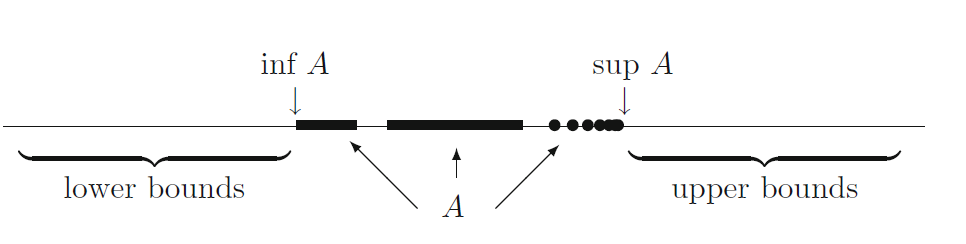
\includegraphics[width=\textwidth]{sup-inf}
  \caption{Definition of $\sup A$ and $\inf A$ \cite{abbott2001understanding}}
  \label{fig:sup-inf}
\end{figure}

%These concepts induces our first definition of real numbers.
%
%\begin{definition}[Real Numbers]
%	The field of \textbf{real numbers} is an ordered field $\textbf{R}$ with the property that given any non-empty subset $A \subset \textbf{R}$ which is bounded above, there exists $\sup A \in \textbf{R}$.
%\end{definition}
%
%The definition above is equivalent to the axiom of completeness. 

The natural question now is: when does the supremum/infimum exist?

\textbf{Axiom of Completeness.} Every non-empty set of real numbers that is bounded above has a least upper bound.

%\begin{definition}[Least-Upper-Bound Property]
%  If \(E \subseteq S\), \(E \neq \emptyset\) and \(E\) is bounded above,
%then \(\sup E\) exists in \(S\) and $S$ is said to have the \textbf{least-upper-bound property}.
%\end{definition}

%\begin{theorem}[]
%Suppose \(S\) is an ordered set with the least-upper-bound property,
%\(B \subseteq S\), \(B\) is not empty, and \(B\) is bounded below. Let
%\(L\) be the set of all lower bounds of \(B\). Then \(\alpha = \sup L\)
%exists in \(S\), and \(\alpha = \inf B\). In particular, \(\inf B\)
%exists in \(S\).
%\end{theorem}
%
%\begin{theorem}[Real Numbers]
%  There exists an ordered field $\textbf{R}$ which has the least-upper-bound property. Moreover, $\textbf{Q}$ contains $\textbf{Q}$ as a subfield.
%\end{theorem}

%% PROOF: Lecture 8, Rudin's appendix

The following theorem is an important property of the real numbers. It states that no matter how large $y$ is and how small $x$ is, if one keeps adding $x$ to itself, one will eventually overtake $y$.

\begin{theorem}[Archimedean Property]
  Let $x, y \in \textbf{R}$, and $x > 0$. Then there exists a positive integer $n$ such that $nx > y$.
\end{theorem}

\begin{proof}[Proof by contradiction.]
	Suppose that there is $a,b > 0$ such that $na \leq b$, $\forall n \in \textbf{N}$. We define \[ S = \{ n \cdot a : n \in \textbf{N} \} \]
	
	In this case, $b$ is an upper bound of $S$. Using the supremum axiom, let $s_0 = \sup S$.
	
	Given that $a > 0$, we have $s_0 < s_0 + a$, hence $s_0 - a < s_0$.
	
	Since $s_0$ is the least upper bound of $S$, $s_0 - a$ can not be an upper bound of $S$. Therefore, $s_0 - a < n_0 a$ for some $n_0 \in \textbf{N}$.
	
	Hence, $s_0 - a < n_0 a$. Which means that $s_0 < n_0 a + a = (n_0 + 1) a$.
	
	Notice that we obtained $(n_0 + 1)a \in S$ and $s_0$ is not an upper bound of $S$, which is a contradiction.
\end{proof}

As a consequence, for every $a \in \textbf{R}_+$, there exists $n \in \textbf{N}$ such that $n a > 1$, i.e., $1/n < a$.

The theorem following states that between any two real numbers there is a rational one.

\begin{theorem}[$\textbf{Q}$ is dense in $\textbf{R}$]
  Given any two real numbers $x < y$, we can find a rational number $q$ such that $x < q < y$.
\end{theorem}

\begin{proof} 
	Exercise. %P. 20 of Abbott, p. 9 of Rudin
\end{proof}

\begin{theorem}[Existence of $n^\text{th}$ roots]
  Let $x$ be a positive real number, and let $n$ be a positive integer. Then there is one and only one positive real number $z$ such that $z^n = x$. This number $z$ is written $\sqrt[n]{x}$ or $x^{1/n}$.
  
  In other words, then the set $E := \{y \in \textbf{R} : y \geq 0 \land y^n \leq x \}$ is non-empty and is also bounded above. In particular, $x^{1/n}$ is a positive real number.
\end{theorem}

%\begin{example}
%	\[ \textbf{R}(X) = \left\lbrace \frac{p(x)}{q(x)} : p(x), q(x) \in \textbf{R}[x], q(x) \neq 0 \right\rbrace \]
%	is an ordered field. Moreover, $\textbf{R} \subset \textbf{R}(x)$ and $f(x) = x$ is bigger than any real number.
%\end{example}

We will end this section with two important propositions about least upper bounds.

\begin{proposition}[Uniqueness of least upper bound]
  Let $E \subseteq \textbf{R}$. Then $E$ can have at most one least upper bound.
\end{proposition}

\begin{proof}
  Let $M_1$ and $M_2$ be two least upper bounds. Given that $M_1$ is a least upper bound and $M_2$ is an upper bound, then by definition of the least upper bound we have $M_2 \geq M_1$. Similarly, since $M_2$ is a least upper bound and $M_1$ is an upper bound, then $M_1 \geq M_2$. Hence, $M_1 = M_2$. 
\end{proof}

\begin{theorem}[Existence of least upper bound]
  Let $E$ be a non-empty subset of $\textbf{R}$. If $E$ has an upper bound, then it must have exactly one least upper bound.
\end{theorem}

\begin{proof}
  Let $M$ be an upper bound of $E$. By the uniqueness of the least upper bound, we know that $E$ has at most one least upper bound. We want to show that $E$ has at least one least upper bound.

  Given that $E$ is non-empty, we can choose some $x_0 \in E$. Let $n \geq 1$ be a positive integer. By the Archimedean property, we can find $K \in \textbf{Z}$ such that $K/n \geq M$, and hence $K/n$ is also an upper bound for $E$.
  
  Using the Archimedean property again, there exists $L \in \textbf{Z}$ such that $L/n < x_0$. Since $x_0 \in E$, $L/n$ is not an upper bound for $E$. Given that $K/n$ is an upper bound but $L/n$ is not, we have $K \geq L$. 

  With that, we can find an integer $L < m_n \leq K$ with the property that $m_n / n$ is an upper bound for $E$, but $(m_n-1)/n$ is not. In fact, $m_n$ is unique. This gives a well-defined and unique sequence $m_1, m_2, m_3, \ldots$ of integers with the property above. 

  Now let $N \geq 1$ be a postive integer, and let $n, n' \geq N$. Since $m_n/n$ is an upper bound for $E$ and $m_{n'}-1/n'$ is not, we have $m_n/n > m_{n'}-1/n'$. This implies that 
  \[
    \frac{m_n}{n} - \frac{m_{n'}}{n'} > - \frac{1}{n'} \geq - \frac{1}{N}
  \]

  Similarly, since $m_{n'}/n'$ is an upper bound for $E$ and $m_{n}-1/n$ is not, we have $m_{n'}/n' > m_{n}-1/n$, and hence
  \[
    \frac{m_n}{n} - \frac{m_{n'}}{n'} \leq \frac{1}{n} \leq \frac{1}{N}
  \]

  Putting these two bounds together,
  \[
    \left| \frac{m_n}{n} - \frac{m_{n'}}{n'} \right | \leq \frac{1}{N} \text{ for all } n,n' \geq N \geq 1
  \]

  This implies that $\frac{m_n}{n}$ is a Cauchy sequence. Since they are rational numbers, we can define the real number $S$ as
  \[
    S := \lim_{n \to \infty} \frac{m_n}{n}
  \]

  Hence,
  \[
    S = \lim_{n \to \infty} \frac{m_n - 1}{n}
  \]

  Now we need to show that $S$ is the least upper bound for $E$.

  Let $x \in E$. Given that $m_n/n$ is an upper bound for $E$, we have $x \leq m_n/n$ for all $n \geq 1$. Therefore, $x \leq \lim_{n \to \infty} \frac{m_n}{n} = S$. Thus $S$ is an upper bound for $E$.

  Suppose that $y$ is an upper bound for $E$. Since $(m_n - 1)/n$ is not an upper bound, $y \geq (m_n - 1)/n$. Hence, $y \geq \lim_{n \to \infty} \frac{m_n - 1}{n} = S$. Thus the upper bound $S$ is less than or equal to every upper bound of $E$, and $S$ is thus a least upper bound of $E$. 
\end{proof}

\newpage
\section{Sequences of Real Numbers}

\subsection{Sequences}

\begin{definition}[Sequence]
	A \textbf{sequence} is a function $f$ defined on the set $\textbf{N}$. If $f(n) = x_n$, $n \in \textbf{N}$, we denote the sequence $f$ by the symbol $(x_n)_{n=1}^\infty$ or, simply, $( x_n )$. The elements $x_n$ are called the \textbf{terms} of the sequence.
	
	Intuitively, a sequence of real numbers is a collection of reals \[a_m, a_{m+1}, a_{m+2}, \ldots\]
	
	If $A$ is a set and if $x_n \in A$ for all $n \in \textbf{N}$, then $\{ x_n \}$ is said to be a \textbf{sequence of elements of $A$}.
\end{definition}

\begin{definition}[Convergence]
	A real sequence $(x_n)$ is said to \textbf{converge} if there is a point $a \in \textbf{R}$ satisfying that for every $\varepsilon > 0$, there exists $n_0 \in \textbf{N}$ such that 
	\[ | x_n -a | < \varepsilon \]
	whenever $n > n_0$.
	
	We also say that $(x_n)$ converges to $a$ or that $a$ is the limit of $(x_n)$, and we write $x_n \longrightarrow a$ or $\lim x_n = a$.
	
	If $(x_n)$ does not converge, then we say that the sequence \textbf{diverges}.
\end{definition}

\begin{definition}[$\varepsilon$-neighbourhood]
	An \textbf{$\varepsilon$-neighbourhood} of $a$, or the neighbourhood of center $a$ and radius $\varepsilon$ is defined as
	\[ V_\varepsilon (a) = \{ x \in \textbf{R} : | x - a | < \varepsilon \} = (a-\varepsilon, a+ \varepsilon) \]
\end{definition}

With this definition, we can understand convergence as follows:
\[
	x_n \longrightarrow a \text{ if } \forall \varepsilon > 0 \, \exists n_0 \in \textbf{N} \text{ such that } x_n \in V_\varepsilon (a), \forall n > n_0
\]

\begin{proposition}[Uniqueness of the limit]
	If $a$ and $b$ are limits of $(x_n)$, then $a=b$.
\end{proposition}

\begin{proof}
	Let $\varepsilon > 0$. Given that $a$ and $b$ are limits of $(x_n$, then there exists $n_1$, $n_2$ such that
	\[
		| x_n - a | < \frac{\varepsilon}{2} \text{ for all } n > n_1
	\]
	\[
		| x_n - b | < \frac{\varepsilon}{2} \text{ for all } n > n_2
	\]
	
	Now let $n_0 = \max \{ n_1, n_2 \}$. Then
	\[
		| b - a | = | b - x_n + x_n - a | \leq |x_n - b| + |x_n - a| < \frac{\varepsilon}{2} + \frac{\varepsilon}{2} = \varepsilon
	\]
	whenever $n > n_0$. Since $\varepsilon$ is arbitrarily small, $|b-a| = 0$. Hence, $a = b$. 
\end{proof}

\begin{definition}
	A sequence is \textbf{upper bounded} if there exists $b \in \textbf{R}$ such that $x_n \leq b$ for all $n \in \textbf{N}$.
	
	A sequence is \textbf{lower bounded} if there exists $a \in \textbf{R}$ such that $x_n \geq a$ for all $n \in \textbf{N}$.
	
	If a sequence is upper bounded and lower bounded, then the sequence is said to be \textbf{bounded}. In this case, there exists an $M \geq 0$ such that $| x_n | \leq M$, i.e., $x_n \in (-M, M)$ for all $n \in \textbf{N}$.
\end{definition}

\begin{proposition}
	Every convergent sequence is bounded.
\end{proposition}

\begin{proof}
	Let $a = \lim x_n$ and take $\varepsilon = 1$. Hence, there exists $n_0 \in \textbf{N}$ such that for all $n > n_0$ we have $x_n \in (a-1, a+1)$. 
	
	Therefore, our task is to `control' the following finite set: \[ I = \{ x_1, x_2, \ldots, x_{n_0} \} \cup \{a-1\} \cup \{a+1\} \]
	
	Let $b$ the smallest value of $I$ and $c$ the biggest value of $I$. Then every term of $(x_n)$ is in the interval $[ b, c ]$.
\end{proof}

The contrapositive of this proposition consists in an useful criteria for the study of the convergence of sequences.

\begin{example}
	The sequence $1,2,3,4,\ldots$ is not bounded. Hence, it is not convergent.
\end{example}

\begin{example}
	The sequence $1,-1,1,-1, \ldots$ is bounded. However, it is not convergent.
\end{example}

\begin{definition}
	A sequence $(x_n)$ is \textbf{non-decreasing} if $x_n \leq x_{n+1}$ for all $n \in \textbf{N}$. And $(x_n)$ is \textbf{non-increasing} if $x_n \geq x_{n+1}$ for all $n \in \textbf{N}$.
	
	If the sequence is non-decreasing or non-increasing, then it is said to be \textbf{monotone}.
\end{definition}

\begin{proposition}
	If a sequence is non-decreasing and upper bounded, then it is convergent. 
\end{proposition}

\begin{proof}
	Let $(x_n)$ be a non-decreasing sequence and upper bounded, and let $b = \sup\{ x_n : n \in \textbf{N} \}$, which is valid by the Axiom of Completeness. We're going to show that $x_n \longrightarrow b$.
	
	Given $\varepsilon > 0$, since $b$ is the least upper bound, there is $n_0 \in \textbf{N}$ such that $b - \varepsilon < x_{n_0}$.
	
	Since the sequence is non-decreasing,
	\[ b - \varepsilon < x_{n_0} \leq x_n, \, \forall n > n_0 \]
	
	Hence,
	\[ b - \varepsilon < x_n < b + \varepsilon \]
	
	Which means that $|x_n - b| < \varepsilon$, for all $n > n_0$. I.e., $x_n \longrightarrow b$.
\end{proof}

Analogously, if a sequence is non-increasing and lower bounded, then it is convergent.

Another way of stating the fact above is that every bounded monotone sequence is convergent.

The following proposition states that if a sequence has a positive limit, then, after a finite number of terms, all of its terms will be positive.

\begin{proposition}
	If $\lim x_n = a > 0$, then there exists $n_0 \in \textbf{N}$ such that $x_n > 0$ whenever $n > n_0$.
\end{proposition}
\begin{proof}
	Let $\varepsilon = a/2 > 0$. Then $(a-\varepsilon, a+\varepsilon) = (a/2, 3a/2)$. There exists $n_0 \in \textbf{N}$ such that if $n > n_0$, then $x_n \in (a/2, 3a/2)$, i.e., $x_n > a/2$. Hence, $x_n > 0$ if $n > n_0$.
\end{proof}

\begin{corollary}
	Let $(x_n)$ and $(y_n)$ be convergent sequences. If $x_n \leq y_n$ for all $n \in \textbf{N}$, then $\lim x_n \leq \lim y_n$.
\end{corollary}
\begin{proof}
	If $\lim x_n > \lim y_n$, we would have \[ 0 < \lim x_n - \lim y_n = \lim (x_n - y_n) \] which implies that $x_n - y_n > 0$ for every $n$ sufficiently big.
\end{proof}

\begin{corollary}
	Let $(x_n)$ be a convergent sequence. If $x_n \geq a$ for all $n$, then $\lim x_n \geq a$.
\end{corollary}

\begin{lemma}\label{zeroandbound}
	If $\lim x_n = 0$ and $(y_n)$ is bounded, then $\lim x_n y_n = 0$.
\end{lemma}

\begin{proof}
	Since $(y_n)$ is bounded, there exists $c > 0$, such that $|y_n| \leq c$, for all $n \in \textbf{N}$. And since $\lim x_n = 0$, we can take $|x_n - 0| = |x_n|$ as small as we want.
	
	Hence, given $\varepsilon > 0$, there exists $n_0 \in \textbf{N}$ such that $|x_n| < \varepsilon / c$, for all $n > n_0$.
	
	Therefore, for all $n > n_0$, 
	\[
		|x_n y_n - 0| = |x_n| |y_n| < \frac{\varepsilon}{c} \cdot c = \varepsilon
	\]
\end{proof}

\begin{example}
	\[ \lim \frac{(-1)^n}{n} = \lim \left( (-1)^n \cdot \frac{1}{n} \right) = 0 \]
\end{example}

\begin{theorem}[Squeeze theorem]
	Let $x_n \leq y_n \leq z_n$ for all $n \in \textbf{N}$. If $\lim x_n = \lim z_n = L$, then $\lim y_n = L$.
\end{theorem}

\begin{proof}
	Given $\varepsilon > 0$, there exists $n_1 \in \textbf{N}$ such that $|x_n - L| < \varepsilon$, for all $n > n_1$. Analogously, there exists $n_2 \in \textbf{N}$ such that $|z_n - L| < \varepsilon$, for all $n > n_2$.
	
	Let $n_0 = \max \{n_1, n_2\}$. By hypothesis, $x_n \leq y_n \leq z_n$, for all $n \in \textbf{N}$. Therefore, for $n > n_0$, \[ L - \varepsilon < x_n \leq y_n \leq z_n < L + \varepsilon \]
	
	That means that $|y_n - L| < \varepsilon$ for all $n > n_0$.
\end{proof}

\begin{example}
	Compute $\lim \frac{\sin n}{n}$.
	
	Since $-1 \leq \sin n \leq n$, we have \[ \frac{-1}{n} \leq \frac{\sin n}{n} \leq \frac{1}{n} \] for all $n \in \textbf{N}$.
	
	But $\lim \frac{-1}{n} = \lim \frac{1}{n} = 0$. Therefore, by the Squeeze theorem, \[ \lim \frac{\sin n}{n} = 0 \]
\end{example}

\subsection{Subsequences}

\begin{definition}[Subsequence]
	Let $(x_n)$ be a sequence. A \textbf{subsequence} of $(x_n)$ is a sequence of the form $(x_{n_j})_{j=1}^\infty$, where $n_j$ is a strictly increasing sequence in $\textbf{N}$. 
\end{definition}

\begin{proposition}
	If $\lim x_n = x$ then every subsequence of $(x_n)$ converges to $x$.
\end{proposition}

\begin{proof}
	Consider $(x_{n_j})_{j=1}^\infty$ a subsequence of $(x_n)$. By hypothesis, $x_n \longrightarrow x$. Therefore, given $\varepsilon > 0$, there exists $n_0 \in \textbf{N}$ such that $|x_n - x| < \varepsilon$, for all $n > n_0$.
	
	Given that the sequence of the index $n_j$ is strictly increasing, there is $j_0 \in \textbf{N}$ such that $n_{j_0} > n_0$. Hence, for all $j > j_0$, \[ | x_{n_j} - x | < \varepsilon \]
\end{proof}

The contrapositive of this proposition is also an useful criteria for studying convergence.

\begin{example}
	The sequence $x_n = (-1)^n$ does not converge, since $x_{2n} \longrightarrow 1$ and $x_{2n-1} \longrightarrow -1$.
\end{example}

Before proving the Bolzano-Weierstrass theorem, which is one of the most important results in Real Analysis, we will prove the following result.

\begin{theorem}[Nested intervals]\label{nested-intervals}
	Let $([a_n, b_n])_{n=1}^\infty$ be a non-increasing sequence of bounded and closed intervals, i.e., \[ [a_1, b_1] \supset [a_2, b_2] \supset \ldots \]
	
	Then, there exists $c \in \textbf{R}$ which belongs to all intervals $[a_n, b_n]$.
\end{theorem}

\begin{proof}
	Since the sequence of intervals is non-increasing, we have
	\[
		a_1 \leq a_2 \leq a_3 \leq \ldots \leq a_n \leq \ldots \leq b_n \leq \ldots \leq b_2 \leq b_1
	\]
	
	Consider the set $A = \{ a_n : n \in \textbf{N} \}$. Given that $A$ is upper bounded and non-empty, let $c = \sup A$. Then $a_n \leq c \leq b_n$ for all $n \in \textbf{N}$. Which means that $c \in [a_n, b_n]$ for all $n \in \textbf{N}$.
\end{proof}

\begin{theorem}[Bolzano-Weierstrass]\label{bolz-weier}
	Every bounded sequence has a convergent subsequence.
\end{theorem}

\begin{proof}
	Let $(a_n)$ be a bounded sequence. Then there exists $M > 0$ such that $|a_n| \leq M$, for all $n \in \textbf{N}$.
	
	Divide the interval $[-M,M]$ into the halves $[-M,0]$ and $[0,M]$. Notice that at least one of the intervals contains infinite terms of the sequence $(a_n)$. Choose the half that contains infinite terms and denote it by $I_1$. Let $a_{n_1}$ a point of the sequence $(a_n)$ such that $a_{n_1} \in I_1$.
	
	Divide $I_1$ into two closed intervals with the same length and let $I_2$ be the half that contains infinite terms. Choose $a_{n_2}$ from the original sequence with $n_2 > n_1$.
	
	In the general case, define $I_k$ by dividing $I_{k-1}$ into two halves and take $I_k$ to be the half with infinite terms of $(a_n)$. Then select $n_k > n_{k-1} > \ldots > n_2 > n_1$ such that $a_{n_k}\in I_k$. 
	
	Now let us show that the subsequence $(a_{n_k})$ is convergent. Notice that $I_1 \supset I_2 \supset \ldots$ is a sequence of closed and nested intervals. By the \hyperref[nested-intervals]{nested intervals theorem}, there exists $x \in \textbf{R}$ which belong to $I_k$, for all $k \in \textbf{N}$. 
	
	Affirmation: $(a_{n_k})$ converges to $x$. 
	
	Let $\varepsilon > 0$. By construction, the length of $I_k$ is equal to $M \left( \frac{1}{2} \right)^k$. Using the Lemma \ref{zeroandbound}, 
	\[
		\lim_{k \to \infty} M \left( \frac{1}{2} \right)^k = 0
	\]
	
	Hence, there exists $n_0 \in \textbf{N}$ such that for all $k > n_0$ the length of $I_k$ is lesser than $\varepsilon$. Since $x$ and $a_{n_k}$ are in $I_k$, we have that the distance $|a_{n_k} - x| < \varepsilon$ for all $k > n_0$.
\end{proof}

We now state some important properties of limits, which will ease their computations. 

\begin{theorem}
	If $\lim a_n = a$ and $\lim b_n = b$, then:
	\begin{enumerate}
		\item $\lim (c \cdot a_n) = c \cdot a$, $\forall c \in \textbf{R}$.
		\item $\lim (a_n + b_n) = a + b$.
		\item $\lim a_n b_n = ab$.
		\item $\lim \left( \frac{a_n}{b_n} \right) = \frac{a}{b}$ if $b \neq 0$.
	\end{enumerate}
\end{theorem}

\begin{proposition}
	A monotone sequence is bounded iff. it has a bounded subsequence.
\end{proposition}

\begin{proof}
	Consider $x_{n_j} \leq b$ a bounded subsequence of the non-decreasing sequence $(x_n)$. Then, for all $n \in \textbf{N}$, there exists $n_k > n$, hence, $x_n \leq x_{n_k} \leq b$. Hence, $x_n \leq b$ for all $n$. 
\end{proof}

\subsection{Cauchy Sequences}

\begin{definition}
	A sequence $(a_n)$ is said to be a \textbf{Cauchy sequence} if for all $\varepsilon > 0$, there is $n_0 \in \textbf{N}$ such that 
	\[
		| a_n - a_m | < \varepsilon
	\]
	for all $n,m > n_0$. Intuitively, this means that after a certain point, every pair of terms are close to each other.
\end{definition}

With that definition, our goal is to show that a real sequence is convergent iff. it is a Cauchy sequence. This is known as the \textbf{Cauchy criterion}.

\begin{lemma}
	Every Cauchy sequence is bounded.
\end{lemma}

\begin{proof}
	Let $\varepsilon = 1$. Then, there exists $n_0$ such that $|x_n - x_m| < 1$ for all $n,m > n_0$. Notice that
	\[ |x_n| = |x_n - x_{n_0+1} + x_{n_0+1}| \leq |x_n - x_{n_0+1}| + |x_{n_0+1}| < 1 +  |x_{n_0+1}| \]
	for all $n > n_0$.
	
	Let $c = \max \{|x_1|, |x_2|, \ldots, |x_{n_0}|, 1+|x_{n_0+1}|\}$. Then $|x_n| \leq c$ for all $n \in \textbf{N}$.
\end{proof}

%\begin{lemma}
%  Every Cauchy sequence $(a_n)_{n=1}^\infty$ is bounded.
%\end{lemma}
%
%\begin{proof}
%  Since $(a_n)_{n=1}^\infty$ is a Cauchy sequence, $a_n$ is an eventually $1$-steady and thus can be split into a finite sequence and a $1$-steady sequence, i.e., there is an $N \geq 0$ such that $|a_j - a_k| \leq 1$ for $j, k \geq N$.
%  
%  For the finite sequence, just apply the prior lemma, returning a boundary $M \geq 0$.
%
%  For the $1$-steady sequence, for all $j,k \geq N$ we have $|a_j - a_k| \leq 1$. Let $k = N$, $x = a_j - a_N$ and $y = a_N$. Then,
%  \[
%    | x + y | - | y | \leq |x| \iff |a_j| - |a_N| \leq |a_j - a_N| \leq 1
%  \]
%  
%  Hence,
%  \[
%    |a_j| \leq 1 + |a_N| \text{ for all } j \geq N
%  \]
%  which gives us the bound to the infinite tail of the sequence.
%
%  Finally, to find the bound over all the sequence, take $M' = M + 1 + |a_N|$. If $1 \leq n < N$, then $|a_n| \leq M \leq M'$. If $n \geq M$, then $|a_n| \leq 1 + |a_N| \leq M'$.
%\end{proof}

\begin{theorem}
	A sequence is convergent if, and only if, it is a Cauchy sequence.
\end{theorem}

\begin{proof}
	$(\Rightarrow)$ Let $(x_n)$ convergent and $\lim x_n = x$. Then, given $\varepsilon > 0$, there exists $n_0 \in \textbf{N}$ such that $|x_n - x| < \varepsilon/2$ for all $n > n_0$. Therefore,
	\[
		|x_n - x_m| = |x_n - x + x - x_m| \leq |x_n - x| + |x_m - x| < \frac{\varepsilon}{2} + \frac{\varepsilon}{2} = \varepsilon, \, \forall n,m > n_0
	\]
	
	$(\Leftarrow)$ Suppose that $(x_n)$ is a Cauchy sequence. Then $(x_n)$ is bounded. By the \hyperref[bolz-weier]{Bolzano-Weierstrass theorem}, $(x_n)$ has a convergent subsequence $(x_{n_k})$. Let $x = \lim x_{n_k}$. We're going to show that the original sequence also converges to $x$.
	
	Let $\varepsilon > 0$. Since $(x_n)$ is a Cauchy sequence, there is $n_0 \in \textbf{N}$, such that $|x_n - x_m| < \varepsilon/2$ for all $n,m > n_0$.
	
	Now, since $(x_{n_k}) \longrightarrow x$, there exists $n_k > n_0$ such that $|x_{n_k} - x| < \varepsilon/2$ for all $n > n_k$.
	
	Hence, for all $n > n_k$, 
	\[
		|x_n - x| = |x_n - x_{n_k} + x_{n_k} - x| \leq |x_n - x_{n_k}| + |x_{n_k} - x| < \frac{\varepsilon}{2} + \frac{\varepsilon}{2} = \varepsilon
	\]
\end{proof}

With Cauchy sequences, Georg Cantor gave another construction of the real numbers $\textbf{R}$.

\begin{definition}[$\varepsilon$-close Sequences]
  Consider two sequences $(a_n)_{n=0}^\infty$ and $(b_n)_{n=0}^\infty$, and let $\varepsilon > 0$. These two sequences are said to be \textbf{$\varepsilon$-close} iff. $a_n$ is $\varepsilon$-close to the sequence $b_n$, for each $n \in \textbf{N}$. I.e., $|a_n - b_n| \leq \varepsilon$ for all $n \in \textbf{N}$.

  If there exists an $N \geq 0$ such that $|a_n - b_n| \leq \varepsilon$ for all $n \geq \textbf{N}$, then the two sequences are said \textbf{eventually $\varepsilon$-close sequences}.
\end{definition}

\begin{definition}[Equivalent Sequences]
  Two sequences are \textbf{equivalent} iff. for each rational $\varepsilon > 0$, the sequences are eventually $\varepsilon$-close.
\end{definition}

%\begin{proposition}
%  Let $(a_n)_{n=1}^\infty$ and $(b_n)_{n=1}^\infty$ be the sequences $a_n = 1 + 10^{-n}$ and $b_n = 1 - 10^{-n}$. Then the sequences $a_n$ and $b_n$ are equivalent.
%\end{proposition}

\begin{definition}[Real numbers]
  A \textbf{real number} is an object of the form
  \[
    \lim_{n \to \infty} a_n
  \]
  where $(a_n)_{n=1}^\infty$ is a Cauchy sequence of rational numbers. Two real numbers $\lim_{n \to \infty} a_n$ and $\lim_{n \to \infty} b_n$ are said to be equal iff. $(a_n)_{n=1}^\infty$ and $(b_n)_{n=1}^\infty$ are equivalent Cauchy sequences.
\end{definition}

\subsection{Upper and Lower Limits}

\begin{definition}
	Let $(x_n)$ be a sequence of real numbers. 
	\begin{itemize}
		\item We say that $(x_n)$ goes to \textbf{infinity} if, for every $N > 0$, there exists $n_0 \in \textbf{N}$ such that $x_n > N$ for all $n > n_0$. We write $x_n \longrightarrow \infty$ or $\lim x_n = \infty$.
		\item We say that $(x_n)$ goes to \textbf{minus infinity} if, given $N > 0$, there exists $n_0 \in \textbf{N}$ such that $x_n < -N$ for all $n > n_0$. We write $x_n \longrightarrow - \infty$ or $\lim x_n = - \infty$.
	\end{itemize}
\end{definition}

\begin{definition}
	Let $(x_n)$ be a sequence of real numbers. Suppose that $(x_n)$ is upper bounded, i.e., $x_n \leq b$ for all $n \in \textbf{N}$.
	
	Define
	\[
		b_n := \sup \{ x_n, x_{n+1}, x_{n+2}, \ldots \} = \sup_{k \geq n} \{ x_k \}
	\]
	Notice that $(b_n)$ is non-increasing. If $(b_n)$ is lower bounded, then $(b_n)$ is convergent. If $(b_n)$ is not lower bounded, then $b_n \longrightarrow - \infty$. 
	
	In both cases, we define \[ \limsup_{n \to \infty} x_n = \lim_n b_n \]
	
	If $(x_n)$ is not upper bounded, then we define \[ \limsup_{n \to \infty} x_n = \infty \]
\end{definition}

\begin{definition}
	Let $(x_n)$ be a sequence of real numbers. Suppose that $(x_n)$ is lower bounded, i.e., $x_n \geq a$ for all $n \in \textbf{N}$.
	
	Define
	\[
		a_n := \inf \{ x_n, x_{n+1}, x_{n+2}, \ldots \} = \inf_{k \geq n} \{ x_k \}
	\]
	Notice that $(a_n)$ is non-decreasing. If $(a_n)$ is upper bounded, then $(a_n)$ is convergent. If $(a_n)$ is not upper bounded, then $a_n \longrightarrow \infty$. 
	
	In both cases, we define \[ \liminf_{n \to \infty} x_n = \lim_n a_n \]
	
	If $(x_n)$ is not lower bounded, then we define \[ \liminf_{n \to \infty} x_n = - \infty \]
\end{definition}	

\begin{example}
	Consider $x_n = (-1)^n$, $n \in \textbf{N}$. Then $b_1 = 1, b_2 = 1, \ldots, b_n = 1$. Hence, $\limsup x_n = \lim b_n = 1$.
	
	And $a_n = -1$, for all $n \in \textbf{N}$. Hence, $\liminf x_n = \lim a_n = -1$.
\end{example}

\begin{example}
	Let $x_n = \frac{(-1)^n}{n}$. Then $\limsup x_n = \lim b_n = 0$, and $\liminf x_n = \lim a_n = 0$.
\end{example}

\begin{example}
	Let $x_n = (-1)^n n$. Then $\limsup x_n = \infty$, and $\liminf x_n = - \infty$.
\end{example}

\begin{remark}
	$a_n \leq b_n$ and therefore $\liminf x_n \leq \limsup x_n$.
\end{remark}

\begin{theorem}
	Let $(x_n)$ be a sequence. Then
	\[
		\lim x_n = L \iff \limsup x_n = \liminf x_n = L
	\]
\end{theorem}

\begin{proof}
	Suppose that $L \in \textbf{R}$.
	
	$(\Rightarrow)$ Suppose that $\lim x_n = L$. Given $\varepsilon > 0$, there exists $n_0 \in \textbf{N}$ such that $L - \varepsilon < x_n < L + \varepsilon$, for all $n > n_0$.
	
	Notice that
	\[
		b_n = \sup_{k \geq n} \{ x_k \} \leq L + \varepsilon, \, \forall n > n_0
	\]
	
	On the other hand,
	\[
		a_n = \inf_{k \geq n} \{ x_k \} \geq L - \varepsilon, \, \forall n > n_0
	\]
	
	Then,
	\[
		L - \varepsilon \leq a_n \leq b_n \leq L + \varepsilon, \, \forall n > n_0
	\]
	
	Hence,
	\[
		\limsup x_n = \liminf x_n = L
	\]
	
	$(\Leftarrow)$ By hypothesis, $\lim a_n = \lim b_n = L$. Let $\varepsilon > 0$. Since $(b_n)$ is non-increasing and converges to $L$, there exists $n_1 \in \textbf{N}$ such that
	\[
		\sup_{k \geq n_1} \{ x_k \} = b_{n_1} < L + \varepsilon
	\]
	
	Analogously, $(a_n)$ is non-decreasing and converges to $L$. Then there exists $n_2 \in \textbf{N}$ such that  
	\[
		\inf_{k \geq n_2} \{ x_k \} = a_{n_2} > L - \varepsilon
	\]
	
	Let $n_0 = \max \{n_1, n_2 \}$. Then $L - \varepsilon < x_n < L + \varepsilon$, for all $n > n_0$.
	
	Therefore, $x_n \longrightarrow L$.
	
	If $\lim x_n = \infty$: \textbf{Exercise.}
\end{proof}

\begin{theorem}
	Let $(x_n)$ a bounded sequence of real numbers. And let $a = \liminf x_n$ and $b = \limsup x_n$.
	
	Then there exists a subsequence $(x_{n_k}) \longrightarrow a$ and a subsequence $(x_{n_j}) \longrightarrow b$.
\end{theorem}

\begin{proof}
	\textbf{Exercise.}
\end{proof}

\subsection{Infinite Series}

In this section, we are going to discuss the meaning of infinite sums like
\[
	\frac{1}{2} + \frac{1}{4} + \ldots + \frac{1}{2^n} + \ldots = 1
\]
and give meaning to this equality.

This infinite sum is called a \textbf{series}, and the main interest in the study of series is whether or not the series converges. To compute to which value it converges is often a cumbersome task and will not be our primary concern.

\begin{definition}
	Let $(a_n)$ be a sequence. An \textbf{infinite series} is defined as
	\[
		\sum_{n=1}^\infty a_n = a_1 + a_2 + a_3 + \ldots
	\]
	
	The sequence $(s_m)$, defined as
	\[
		s_m = a_1 + a_2 + \ldots + a_m
	\]
	is called the \textbf{sequence of partial sums}.
	
	And the series $\sum_{n=1}^\infty$ \textbf{converges} to $A$ if the sequence $(s_m)$ converges to $A$, and we write $\sum_{n=1}^\infty = A$.
\end{definition}

\begin{example}[Harmonic Series]
	Consider the \textbf{harmonic series}
	\[
		\sum_{n=1}^\infty \frac{1}{n}
	\]
	
	Since the sequence of partial sums
	\[
		s_m = 1 + \frac{1}{2} + \ldots + \frac{1}{m}
	\]
	is increasing and unbounded, this series does not converge. 
\end{example}

\begin{theorem}
	If $\sum_{n=1}^\infty a_n = A$ and $\sum_{n=1}^\infty b_n = B$, then
	\begin{enumerate}
		\item $\sum_{n=1}^\infty c a_n = cA$ for all $c \in \textbf{R}$.
		\item $\sum_{n=1}^\infty (a_n + b_n) = A + B$.
	\end{enumerate}
\end{theorem}

\begin{theorem}[Cauchy Criterion for Series]
	The series $\sum_{n=1}^\infty a_n$ converges if, and only if, for every $\varepsilon > 0$, there is $N \in \textbf{N}$ such that whenever $n > m > N$ it follows that
	\[
		| a_{m+1} + a_{m+2} + \ldots + a_n | < \varepsilon
	\]
\end{theorem}

\begin{proof}
	Observe that
	\[
		| s_n - s_m | = | a_{m+1} + a_{m+2} + \ldots + a_n | = \left| \sum_{k=m+1}^n a_k \right| < \varepsilon
	\]
	
	Then, using Cauchy criterion for sequences, the result follows immediately. 
\end{proof}

\begin{theorem}
	If the series $\sum_{n=1}^\infty a_n$ converges, then $\lim (a_n) = 0$.
\end{theorem}

\begin{proof}
	Take $n = m+1$ in the previous theorem.
\end{proof}

Notice that the converse of this theorem is not valid. Consider, for example, the harmonic series. 

\begin{theorem}[Comparison Test]
	Suppose that $(a_k)$ and $(b_k)$ are sequences such that $0 \leq a_k \leq b_k$ for all $k \in \textbf{N}$.
	\begin{enumerate}
		\item If $\sum_{k=1}^\infty b_k$ converges, then $\sum_{k=1}^\infty a_k$ converges.
		\item If $\sum_{k=1}^\infty a_k$ diverges, then $\sum_{k=1}^\infty b_k$ diverges.
	\end{enumerate}
\end{theorem}

\begin{proof}
	Let $n > m$. Then $|s_n^a - s_m^a| = |a_{m+1} + \ldots + a_n|$ and $|s_n^b - s_m^b| = |b_{m+1} + \ldots + b_n$. And we have that \[ |a_{m+1} + \ldots + a_n | \leq |b_{m+1} + \ldots + b_n| \]
	
	Now, if $\sum_{k=1}^\infty b_k$ converges, then given $\varepsilon > 0$, there exists $n_0 \in \textbf{N}$ such that $n > m \geq n_0$, we have $|b_{m+1} + \ldots + b_n| < \varepsilon$. And, therefore, $|a_{m+1} + \ldots + a_n| < \varepsilon$ and $\sum_{k=1}^\infty a_k$ converges.
\end{proof}

\begin{example}[Geometric Series]
	A series is called \textbf{geometric} if it is of the form
	\[
		\sum_{n=0}^\infty ax^n = a + ax + ax^2 + ax^3 + \ldots
	\]
	
	If $x = 1$ and $a \neq 0$, then the series diverges. For $x \neq 1$, since
	\[
		(1-x)(1+x+x^2+x^3+\ldots+x^{m-1}) = 1 - x^m 
	\]
	we can write
	\[
		s_m = a + ax + ax^2 + \ldots + ax^{m-1} = \frac{a(1-x^m)}{1-x}
	\]
	
	Hence, 
	\[
		\sum_{n=0}^\infty ax^n = \frac{a}{1-x}
	\]
	if, and only if, $|x| < 1$.
\end{example}

\begin{theorem}[Cauchy Condensation Test]
	Suppose that $(b_n)$ is decreasing and satisfies $b_n > 0$ for all $n \in \textbf{N}$. Then, the series $\sum_{n=1}^\infty b_n$ converges if and only if the series
	\[
		\sum_{n=0}^\infty 2^n b_{2^n} = b_1 + 2b_2 + 4b_4 + 8b_8 + 16b_16 + \ldots
	\]
	converges.
\end{theorem}

\begin{example}
	The series $\sum_{n=1}^\infty \frac{1}{n^p}$ converges if, and only if, $p > 1$.
	
	If $p \leq 0$, then $\lim \frac{1}{n^p} \neq 0$. Therefore, the series diverges.
	
	If $p > 0$, using Cauchy Condensation Test, we can evaluate
	\[
		\sum_{k=0}^\infty 2^k \frac{1}{2^{kp}} = \sum_{k=0}^\infty 2^{(1-p)k}
	\]
	
	Taking $x = 2^{1-p}$ into the geometric series, the series will converge if and only if $1-p < 0$, as we wanted.
\end{example}

\begin{theorem}
	If $\sum_{k=1}^\infty a_k = A$ and $\sum_{k=1}^\infty b_k = B$, then
	\begin{enumerate}
		\item[(i)] $\sum_{k=1}^\infty c a_k = c A$ for all $c \in \textbf{R}$.
		\item[(ii)] $\sum_{k=1}^\infty (a_k + b_k) = A + B$.
	\end{enumerate}
\end{theorem}

\begin{proof}
	(i) Let $t_m = c a_1 + c a_2 + \ldots + c a_m = c (a_1 + \ldots + a_m) = c s_m$. Then \[ \lim t_m = \lim c s_m = c \lim s_m = c A \]
	
	(ii) \textbf{Exercise.}
\end{proof}

\begin{theorem}[Absolute Convergence Test]
	If the series $\sum_{k=1}^\infty |a_k|$ converges, then $\sum_{k=1}^\infty a_k$ also converges.
\end{theorem}

\begin{proof}
	Since $\sum_{k=1}^\infty |a_k|$ converges, by the Cauchy Criterion for Series, given an $\varepsilon > 0$, there exists an $n_0 \in \textbf{N}$ such that
	\[
		|a_{m+1}| + |a_{m+2}| + \ldots + |a_n| < \varepsilon
	\]
	for all $n > m \geq n_0$. By the triangle inequality,
	\[
		|a_{m+1} + a_{m+2} + \ldots + a_n| \leq |a_{m+1}| + |a_{m+2}| + \ldots + |a_n| < \varepsilon
	\]
	By the sufficiency of the Cauchy Criterion, $\sum_{k=1}^\infty a_k$ also converges.
\end{proof}

Notice that the converse is false. Consider the \textbf{alternating harmonic series}
\[
	\sum_{k=1}^\infty \frac{(-1)^{n+1}}{n} = 1 - \frac{1}{2} + \frac{1}{3} - \frac{1}{4} + \ldots
\]

\begin{theorem}[Alternating Series Test]
	Let $(x_k)$ be a sequence such that
	\begin{enumerate}
		\item[(i)] $x_1 \geq x_2 \geq \ldots \geq 0$.
		\item[(ii)] $\lim x_k = 0$.
	\end{enumerate}
	Then, the alternating series $\sum_{k=1}^\infty (-1)^{k+1} a_k$ converges.
\end{theorem}

\begin{proof}
	First, we're going to consider the partial sums of odd indexes. Notice that
	\[
		s_{2n+1} = x_1 - x_2 + x_3 - x_4 + \ldots + x_{2n-1} - x_{2n} + x_{2n+1} = s_{2n-1} - (x_{2n} - x_{2n-1}) \leq s_{2n-1}
	\]
	I.e., $s_{2n-1}$ is non-increasing. On the other hand,
	\[
		s_{2n-1} = (x_1 - x_2) + \ldots + (x_{2n-3} - x_{2n-2}) + x_{2n-1}
	\]
	Which means that $s_{2n-1} \geq 0$. Hence, $(s_{2n-1})$ converges.
	
	Now, we're going to consider the partial sums of even indexes. Notice that
	\[
		s_{2n+2} = x_1 - x_2 + x_3 - x_4 + \ldots + x_{2n-1} - x_{2n} + x_{2n+1} - x_{2n+2} = s_2n + (x_{2n+1} - x_{2n+2}) gleq s_{2n}
	\]
	Which means that $s_{2n}$ is non-decreasing. On the other hand,
	\[
		s_{2n} = x_1 - (x_2 - x_3) - \ldots - (x_{2n-2} - x_{2n-1}) - x_{2n}
	\]
	I.e., $s_{2n} \leq x_1$, for all $n \in \textbf{N}$. Hence, $(s_{2n})$ converges.
	
	Let $L = \lim s_{2n-1}$ and $M = \lim s_{2n}$. Then,
	\[
		\lim (s_{2n} - s_{2n-1}) = \lim (-x_n) = 0
	\]
	and, therefore, $M - L = 0$. Hence, $\lim s_{2n} = \lim s_{2n-1} = L$.
	
	Given $\varepsilon > 0$, there exists $n_1 \in \textbf{N}$ such that $|s_{2n-1} - L| < \varepsilon$ for all $n \geq n_1$. And there exists $n_2 \in \textbf{N}$ such that $|s_{2n} - L| < \varepsilon$ for all $n \geq n_2$.
	
	Fix $k_1 = 2n_1 +1$ and $k_2 = 2n_2$. Let $k_0 = \max \{ k_1, k_2 \}$. Then,
	\[
		|s_k - L| < \varepsilon
	\]
	for all $k > k_0$.
	
	Hence, $\lim s_k = L$ and the series converges.
\end{proof}

\begin{definition}
	If $\sum_{k=1}^\infty |a_k|$ converges, then we say that $\sum_{k=1}^\infty a_k$ \textbf{converges absolutely}. If $\sum_{k=1}^\infty a_k$ converges but the series of absolute values $\sum_{k=1}^\infty |a_k|$ does not converge, then we say that $\sum_{k=1}^\infty a_k$ \textbf{converges conditionally}.
\end{definition}

\begin{lemma}\label{absconvlemma}
	Let $\sum b_n$ be an absolutely convergent series with $b_n \neq 0$ for all $n \in \textbf{N}$ If the sequence $\left( \frac{a_n}{b_n} \right)$ is bounded, then $\sum a_n$ converges absolutely.
\end{lemma}

\begin{proof}
	Suppose that $\left( \frac{a_n}{b_n} \right)$ is bounded, i.e., there exists $c \in \textbf{R}$ such that for all $n \in \textbf{N}$,
	\[
		\left| \frac{a_n}{b_n} \right| \leq c
	\]
	
	Hence, $|a_n| \leq c |b_n|$ for all $n \in \textbf{N}$. By the Comparison Test, $\sum |a_n|$ converges. Therefore, $\sum a_n$ converges absolutely.
\end{proof}

\begin{example}
	Does \[ \sum \frac{1}{n^2 - 3n + 1} \] converges?
	
	Consider $\sum \frac{1}{n^2}$, which is absolutely convergent. And notice that
	\[
	\frac{\frac{1}{n^2 - 3n + 1}}{\frac{1}{n^2}} = \frac{n^2}{n^2-3n+1}
	\]
	is bounded by $1$. Therefore, the series converges.
\end{example}

\begin{theorem}[Ratio Test (D'Alambert)]
	Let $a_n \neq 0$ for all $n \in \textbf{N}$. If there exists $c \in \textbf{R}$ such that
	\[
		\left| \frac{a_{n+1}}{a_n} \right| \leq c < 1
	\]
	for sufficiently large $n$, then the series $\sum a_n$ converges absolutely.
\end{theorem}

\begin{proof}
	Suppose $0 < c < 1$ such that for $n$ sufficiently large, we have
	\[
		\left| \frac{a_{n+1}}{a_n} \right| \leq c = \frac{c^{n+1}}{c^n} \iff \frac{|a_{n+1}|}{c^{n+1}} \leq \frac{|a_n|}{c^n}
	\]
	
	Hence, the sequence of non-negative numbers $\frac{|a_n|}{c^n}$ is non-increasing for $n$ sufficiently large and, therefore, bounded.
	
	Since the series $\sum c^n$ converges absolutely (geometric series), by the \hyperref[absconvlemma]{previous lemma}, $\sum a_n$ converges absolutely.
\end{proof}

\begin{remark}\label{ratiorootremark}
	In general, we compute
	\[
		\lim \left| \frac{a_{n+1}}{a_n} \right| = L
	\]
	\begin{itemize}
		\item If $L < 1$, the series converges.
		\item If $L > 1$, the series diverges. In this case, $|a_{n+1}| > |a_n|$ and hence the general term does not converges to zero.
		\item If $L = 1$, the test implies nothing about the convergence of the series. Consider, for example, $\sum \frac{1}{n^2}$ and $\sum \frac{1}{n}$. Both limits are $1$, but only the first series converges.
	\end{itemize}
\end{remark}

\begin{example}
	Does the series \[ \sum_{n=1}^\infty \frac{n!}{n^n} \] converges?
	
	By the ratio test,
	\begin{equation*}
		\begin{aligned}
			\left| \frac{a_{n+1}}{a_n} \right| &= \frac{(n+1)!}{(n+1)^{(n+1)}} \frac{n^n}{n!} = \frac{(n+1)}{(n+1)^{(n+1)}} n^n = (n+1)^{-n} n^n \\
			&= \left( \frac{n}{n+1} \right)^n = \left( \frac{1}{1+1/n} \right)^n \underset{n \to \infty}{\longrightarrow} \frac{1}{e} < 1
		\end{aligned}
	\end{equation*}
	
	Hence, the series converges.
\end{example}

\begin{theorem}[Root Test (Cauchy)]
	If there exists $c \in \textbf{R}$ such that $\sqrt[n]{|a_n|} \leq c < 1$ for all $n$ sufficiently large, then the series $\sum a_n$ converges absolutely.
\end{theorem}

\begin{proof}
	Suppose that $\sqrt[n]{|a_n|} \leq c < 1$. Then $|a_n| \leq c^n$ for all $n$ sufficiently large. Since $\sum c^n$ converges, it follows from the comparison test that $\sum |a_n|$ converges.
\end{proof}

\begin{remark}
	In general, we compute $\lim \sqrt[n]{|a_n|} = L$ and the previous \hyperref[ratiorootremark]{remark} also applies.
\end{remark}

\begin{example}
	Does the series \[ \sum_{n=1}^\infty \frac{n}{2^n} \] converges?
	
	Notice that
	\[
		\lim \sqrt[n]{\frac{n}{2^n}} = \lim \frac{\sqrt[n]{n}}{\sqrt[n]{2^n}} = \frac{1}{2} < 1
	\]
	
	Hence, the series converges.
\end{example}

\textbf{Exercise.} Show that $\lim \sqrt[n]{n} = 1$.

\subsection{Rearrangements}

Intuitively, a rearrangement of a series is a permutation of its terms into another order.

For example, we know that the series \[ \sum_{n=1}^\infty \frac{(-1)^{n+1}}{n} = 1 - \frac{1}{2} + \frac{1}{3} - \frac{1}{4} + \ldots = p \neq 0 \]

In fact, as we will prove later in this text, $\ln (1+x) = \sum_{n=0}^\infty \frac{(-1)^{n}}{n+1} x^{n+1}$. Hence, $p = \ln (2)$.

The question that motivates this section is: Does changing the order of the terms change the sum?

Notice that
\begin{equation*}
	\begin{aligned}
		p &=  1 - \frac{1}{2} + \frac{1}{3} - \frac{1}{4} + \frac{1}{5} - \frac{1}{6} + \frac{1}{7} - \frac{1}{8} + \frac{1}{9} - \frac{1}{10} + \frac{1}{11} - \frac{1}{12} + \ldots \\
		&= \left( 1 - \frac{1}{2} \right) - \frac{1}{4} + \left( \frac{1}{3} - \frac{1}{6} \right) - \frac{1}{8} + \left( \frac{1}{5} - \frac{1}{10} \right) - \frac{1}{12} + \ldots \\
		&= \frac{1}{2} - \frac{1}{4} + \frac{1}{6} - \frac{1}{8} + \frac{1}{10} - \frac{1}{12} + \ldots = \frac{1}{2} p
	\end{aligned}
\end{equation*}

Hence,
\[
	p = \frac{p}{2} \underset{p \neq 0}{\implies} 1 = 2
\]
which is a contradiction.

This example motivates the following definition.

\begin{definition}[Rearrangement]
	Let $\sum_{k=1}^\infty a_k$ be a series. We say that $\sum_{k=1}^\infty b_k$ is a \textbf{rearrangement} of $\sum_{k=1}^\infty a_k$ if there's a bijection $f: \textbf{N} \longrightarrow \textbf{N}$ such that $b_{f(k)} = a_k$ for all $k \in \textbf{N}$.
\end{definition}

\begin{theorem}
	If a series converges absolutely, then any rearrangement of the series converges to the same limit.
\end{theorem}

\begin{proof}
	Suppose that $\sum_{k=1}^\infty a_k$ converges absolutely to $A \in \textbf{R}$, and let $\sum_{k=1}^\infty b_k$ be a rearrangement of $\sum_{k=1}^\infty a_k$. Define
	\[
		s_n = \sum_{k=1}^n a_k \text{ and } t_m = \sum_{k=1}^m b_k
	\]
	
	We want to show that $\lim t_m = A$. 
	
	Let $\varepsilon > 0$. By hypothesis, $\lim s_n = A$. Hence, choose $N_1 \in \textbf{N}$ such that
	\[
		|s_n - A| < \frac{\varepsilon}{2}
	\]
	for all $n > N_1$. Since the convergence is absolute, we can choose $N_2 \in \textbf{N}$ such that
	\[
		\sum_{k=m+1}^n |a_k| < \frac{\varepsilon}{2}
	\]
	for all $n > m > N_2$.
	
	Notice that $sum_{k=1}^\infty |a_k|$ converges, but not necessarily to $A$. 
	
	Now, let $N = \max \{ N_1, N_2 \}$. We will consider the part of the rearranged series where the terms $\{ a_1, a_2, \ldots, a_N \}$ does not appear. In order to do that, we choose
	\[
		M = \max \{ f(k) : 1 \leq k \leq N \}
	\]
	where $f$ is the function that rearranges the terms.
	
	Since $f$ is injective, $N \leq M$. Let $n \geq M$. Then,
	\[
		\{ a_1, a_2, \ldots, a_N \} \subseteq \{ b_1, b_2, \ldots, b_m \}
	\]
	This means that we moved so far in the rearranged series so that all terms $a_1, \ldots, a_N$ were included. 
	
	Thus, $(t_m - s_N)$ consists of the values such that their absolute value appear in $\sum_{k=N+1}^\infty |a_k|$. Our choice of $N_2$ guarantees that $|t_m - s_N| < \varepsilon / 2$. Then,
	\begin{equation*}
		\begin{aligned}
			|t_m - A| &= |t_m - s_N + s_N - A| \\
			&\leq |t_m - s_N| + |s_N - A| \\
			&< \frac{\varepsilon}{2} + \frac{\varepsilon}{2} = \varepsilon
		\end{aligned}
	\end{equation*}
	whenever $m > M \geq N_2$.
\end{proof}

\textbf{Exercise.} Show that
\[
	\sum_{n=1}^\infty \frac{1}{2n-1} = + \infty \text{ and } \sum_{n=1}^\infty \frac{-1}{2n} = - \infty
\]

The following theorem states that changing conveniently the order of the terms of a conditionally convergent series, it is possible to make its sum to be equal to any given real number.

\begin{theorem}[Riemann]
	Let $\sum a_n$ be a conditionally convergent series and $- \infty \leq a \leq b \leq + \infty$. Then there exists a rearrangement $\sum b_n$, with partial sums $t_n$ such that
	\[
		\liminf_{n \to \infty} t_n = a \text{ and } \limsup_{n \to \infty} t_n = b
	\]
\end{theorem}

\begin{proof}[Idea of the proof]
	Let $\sum a_n$ be a conditionally convergent series. Fix a real number $c > 0$.
	
	We start with the sum of the positive terms $p_n$ of $\sum a_n$ in their original order until the moment that, when we sum $a_n$, the sum goes beyond $c$ for the first time. Notice that this is possible because $\sum p_n = + \infty$.
	
	To this sum, we add the negative terms, also in their natural order, stopping when we sum $a_{n_2}$ such that this sum is lower than $c$.
	
	Repeating this algorithm, we obtain a new series whose terms are the same ones from $\sum a_n$, but in a different order.
	
	Notice that $|s_{n_{k-1}} - c| < a_{n_k}$, where the change of sign happened. Since $\lim a_n = 0$, this new series converges.
\end{proof}

\newpage
\section{Basic Topology of \textbf{R}}

In this section, we are going to go deeper in our previous study of sets, discussing open and closed sets, compact sets, and perfect sets.

\subsection{Open and Closed Sets}

\begin{definition}[Interior point]
	Let $O$ be a subset of $\textbf{R}$. A point $x$ is an \textbf{interior point} of $O$ if there is an $\varepsilon$-neighbourhood of $x$ contained in $O$, i.e., $V_{\varepsilon}(x) \subseteq O$ 
\end{definition}

\begin{definition}[Open set]
	Let $O \subseteq \textbf{R}$. Then $O$ is said to be \textbf{open} if every point $x \in O$ is an interior point of $O$.
\end{definition}

\begin{example}
	\begin{enumerate} \hfill
		\item $\textbf{R}$ is open.
		\item $\emptyset$ is open (vacuously true).
		\item The open interval $(c, d)$ is open. To see that, take $x \in (c,d)$ and take $varepsilon = \min \{ x-c, d-x \}$. Then $V_{\varepsilon}(x) \subseteq (c,d)$. Does this proof remains valid for $(c,d]$?
	\end{enumerate}
\end{example}

\begin{theorem}\label{union-inter-open}
	\begin{itemize} \hfill
		\item[a)] The union of any collection of open sets is open.
		\item[b)] The intersection of a finite collection of open sets is open.
	\end{itemize}
\end{theorem}

\begin{proof}
	\textbf{a)} Let $\{ O_\lambda : \lambda \in \Lambda \}$ be a collection of open sets. Define $O = \bigcup_{\lambda \in \Lambda} O_\lambda$ and $a \in O$. Then $a \in O_{\lambda'}$ for some $\lambda' \in \Lambda$. Since $O_{\lambda'}$ is open, then there exists $\varepsilon > 0$ such that $V_\varepsilon(a) \subseteq O_{\lambda'} \subseteq O$.
	
	\textbf{b)} Let $\{ O_1, \ldots, O_N\}$ be a finite collection of open sets. Define $O = \bigcap_{k=1}^N$ and $a \in O$. Then $a \in O_k$ for all $k = 1, \ldots, N$. Since each $O_k$ is open, there exists $\varepsilon_k > 0$ such that $V_\varepsilon(a) \subseteq O_k$. Take $\varepsilon = \min \{ \varepsilon_1, \ldots, \varepsilon_N \}$. Then
	\[
		V_\varepsilon(a) \subseteq V_{\varepsilon_k}(a) \subseteq O_k
	\]
	for all $k = 1, \ldots, N$. Hence, $V_\varepsilon(a) \subseteq O$.
\end{proof}

\begin{example}
	Let $I_n = \left( \frac{-1}{n}, \frac{1}{n} \right)$, $n \in \textbf{N}$. Then $\bigcap_{n \in \textbf{N}} I_n = \{ 0 \}$ is not open.
\end{example}

\begin{definition}[Limit and isolated points]
	A point $x$ is a \textbf{limit point} (or \textbf{accumulation points}) of a set $A$ if every $\varepsilon$-neighbourhood of $x$ intersects the set $A$ in some point other than $x$.
	
	A point $a \in A$ is an \textbf{isolated point} if $a$ is not a limit point of $A$.
\end{definition}

\begin{theorem}\label{limpointseq}
	A point $x$ is a limit point of a set $A$ if and only if $x = \lim a_n$ for some sequence $(a_n)$ contained in $A$ satisfying $a_n \neq x$ for all $n \in \textbf{N}$.
\end{theorem}

\begin{proof}
	$(\Rightarrow)$ Suppose that $x$ is a limit point of $A$. We are going to construct a sequence such that $a_n \longrightarrow x$.
	
	Since $x$ a limit point, for each $n \in \textbf{N}$ we can choose an element of the set $V_{1/n}(x) \cap A$ other than $x$, which we will call $a_n$.
	
	Given $\varepsilon > 0$, take $N \in \textbf{N}$ such that $1/N < \varepsilon$. Then, for all $n \geq N$.
	\[
		| a_n - x | < \frac{1}{N} < \varepsilon
	\]
	i.e., $a_n \longrightarrow x$.
	
	$(\Leftarrow)$ Assume that $\lim a_n = x$, where $a_n$ is an element of $A$ other than $x$. Let $V_\varepsilon(x)$ be arbitrary. By the definition of convergence, there exists a term $a_N \in V_\varepsilon(x)$.
\end{proof}

Notice that a limit point may not belong to the set $A$.

\begin{definition}[Closed set]
	A set $F \subseteq{R}$ is \textbf{closed} if $F$ contains all of its limit points.
\end{definition}

In Analysis, to be `closed' is with respect to the limiting operation. A closed set is a set where convergent sequences within the set have limits that are also in the set.

\begin{example}
	Consider
	\[
		A = \left\{ \frac{1}{n} : n \in \textbf{N} \right\}
	\]
	
	Each point of $A$ is isolated. In fact, given $1/n \in A$, choose $\varepsilon = \frac{1}{n} - \frac{1}{n+1}$. Then \[ V_\varepsilon(1/n) \cap A = \left\{ \frac{1}{n} \right\} \] Then, $1/n$ is isolated. 
	
	Although all of the points of $A$ are isolated, the set does have one limit point, $0$. Hence, $A$ is not closed. However, the set $F = A \cup \{0\}$ is closed and is called the \textbf{closure} of $A$. 
\end{example}

\begin{example}
	The set $[c,d] = \{ x \in \textbf{R} : c \leq x \leq d \}$ is closed.
	
	In fact, let $x$ be a limit point of $[c,d]$. Then, by the Theorem \ref{limpointseq}, there exists $(x_n) \subseteq [c,d]$ such that $x_n \to x$. We're going to prove that $x \in [c,d]$. Since $c \leq x_n \leq d$, for all $n \in \textbf{N}$, then $c \leq \lim x_n \leq d$. Hence, $[c,d]$ is closed.
\end{example}

\begin{example}
	Consider the set of rational numbers $\textbf{Q} \subseteq \textbf{R}$. The set of limit points of $\textbf{Q}$ is $\textbf{R}$.
	
	Let $y \in \textbf{R}$. Then consider the neighbourhood $V_{\varepsilon}(y) = (y - \varepsilon, y + \varepsilon)$. By the density of $\textbf{Q}$ in $\textbf{R}$, there exists $r \neq y$ such that $r \in V_{\varepsilon}(y)$. Thus, $y$ is a limit point of $\textbf{Q}$.
\end{example}

With the last example, we can restate the density of $\textbf{Q}$ in $\textbf{R}$.

\begin{theorem}[Density of $\textbf{Q}$ in $\textbf{R}$]
	Given $y \in \textbf{R}$, there exists a sequence of rational numbers that converges to $y$. 
\end{theorem}

\begin{definition}[Closure]
	Given a set $A \subseteq \textbf{R}$, let $L$ be the set of all limit points of $A$. The \textbf{closure} of $A$ is defined as $\bar{A} = A \cup L$.
\end{definition}

Notice that a set $F \subseteq \textbf{R}$ is closed if, and only if, every Cauchy sequence contained in $\textbf{R}$ which has a limit, the limit is also in $F$.

\begin{example}
	\begin{enumerate}
		\item If $A = (a,b)$, then $\bar{A} = [a,b]$.
		\item If $A = \textbf{Q}$, then $\bar{A} = \textbf{R}$.
		\item If $A = [a,b]$, then $\bar{A} = [a,b]$.
	\end{enumerate}
\end{example}

\begin{theorem}
	For any $A \subseteq \textbf{R}$, the closure $\bar{A}$ is a closed set and is the smallest closed set containing $A$.
\end{theorem}

\begin{proof}
	Let $L$ denote the set of limit points. Then $\bar{A} = A \cup L$ contains all limit points of $A$.
	
	However, any closed set containing $A$ must contain $L$. Hence, $\bar{A}$ is the smallest closed set containing $A$.
\end{proof}

\begin{definition}[Complement]
	Let $O \subseteq \textbf{R}$. Then the \textbf{complement} of $O$ is defined as
	\[
		O^c = \{ x \in \textbf{R} : x \notin O \}
	\]
\end{definition}

An important relationship between open and closed sets is given by the following theorem.

\begin{theorem}
	A set $O$ is open if, and only if, $O^c$ is closed.
\end{theorem}

\begin{proof}
	Let $O \subseteq \textbf{R}$ be an open set. To show that $O^c$ is closed, we need to prove that $O^c$ contains all of its limit points. If $x$ is a limit point of $O^c$, then every neighbourhood of $x$ contains a point of $O^c$. Now, if $x \in O$, there exists $\varepsilon > 0$ such that $V_{\varepsilon}(x) \subseteq O$, which is not possible. Hence, $x \in O^c$.
	
	Reciprocally, assume that $O^c$ is closed and let $x \in O$. Since $O^c$ is closed, $x$ is not a limit point of $O^c$. By the definition of limit point, there exists $\varepsilon > 0$ such that $V_{\varepsilon}(x)$ does not intersect $O^c$, i.e., $V_{\varepsilon}(x) \subseteq O$, and, hence, $O$ is open.
\end{proof}

\begin{corollary}
	$F$ is closed if, and only if, $F^c$ is open.
\end{corollary}

\begin{proof}
	Follows from the previous proof, observing that $(A^c)^c = A$.
\end{proof}

\begin{theorem}\label{union-inter-closed}
	\begin{itemize} \hfill
		\item[a)] The union of a finite collection of closed sets is closed.
		\item[b)] The intersection of any collection of closed sets is closed.
	\end{itemize}
\end{theorem}

\begin{proof}
	Using DeMorgan's laws, for a collection $\{ E_{\lambda} : \lambda \in \Lambda\}$, we have
	\[
		\left( \bigcup_{\lambda \in \Lambda} E_\lambda \right)^c = \bigcap_{\lambda \in \Lambda} E_\lambda^c \text{ and } \left( \bigcap_{\lambda \in \Lambda} E_\lambda \right)^c = \bigcup_{\lambda \in \Lambda} E_\lambda^c
	\]
	and the result follows immediately by the Theorem \ref{union-inter-open}.
\end{proof}

\subsection{Compact Sets}

Compact sets are generalization of closed intervals.

\begin{definition}[Compactness]
	A set $K \subseteq \textbf{R}$ is \textbf{compact} if every sequence in $K$ has a subsequence that converges to a limit that is also in $K$.
\end{definition}

\begin{example}
	The interval $[c,d]$ is compact. That can be seen by using Bolzano-Weierstrass Theorem, noticing that a closed interval is a closed set.
\end{example}

Generalizing this example, we can obtain an equivalent definition for compactness.

\begin{theorem}[Heine-Borel]\label{heine-borel}
	A set $K \subseteq \textbf{R}$ is compact if, and only if, it is closed and bounded.
\end{theorem}

\begin{proof}
	Suppose that $K$ is compact. First, we'll assume that $K$ is not bounded. Then, there exists $x_1 \in K$ such that $|x_1| > 1$, and $x_2 \in K$ such that $|x_2| > 2$, and, for all $n \in \textbf{N}$ we can produce $x_n \in K$ such that $|x_n| > n$.
	
	Since we assumed that $K$ is compact, $(x_n)$ must have a convergent subsequence $(x_{n_k})$. And since $(x_{n_k})$ is not bounded, $(x_{n_k})$ does not converge. Hence, by contradiction, $K$ must be bounded.
	
	Now, to show that $K$ is closed, let $x = \lim x_n$, with $(x_n) \subseteq K$. We're going to show that $x \in K$. Since $K$ is compact, $(x_n)$ has a convergent subsequence $(x_{n_k})$. Since $K$ is compact and $(x_n) \to x$, we obtain $x \in K$. Hence, $K$ is closed.
	
	To prove the converse statement, suppose that $K$ is bounded and closed and $(x_n) \subseteq K$. By the Bolzano-Weierstrass Theorem, $(x_n)$ has a convergent subsequence $(x_{n_k}) \subseteq K$. Since $K$ is closed, $\lim x_{n_k} = x \in K$. Hence, $K$ is compact.
\end{proof}

\begin{theorem}[Nested Compact Set Property]
	If $K_1 \supseteq K_2 \supseteq K_3 \supseteq \ldots$ is a nested sequence of non-empty compact sets, then the intersection is non-empty.
	\[
		\bigcap_{n=1}^\infty \neq \emptyset
	\]
\end{theorem}

\begin{proof}
	For each $n \in \textbf{N}$, let $x_n \in K_n$. Then $(x_n) \subseteq K_1$ and, since $K_1$ is compact, then there exists a subsequence $(x_{n_k}) \subseteq K_1$ such that $\lim x_{n_k} = x \in K_1$.
	
	Notice that $x \in K_n$ for every $n \in \textbf{N}$. Let $n_0 \in \textbf{N}$. Then, the terms of the sequence $(x_n)$ are in $k_{n_0}$, for all $n \geq n_0$. Ignoring a finite number of terms $n_k < n_0$, the same sequence $(x_{n_k})$ is also contained in $K_{n_0}$ and converges to $x = \lim x_{n_k}$ in $K_{n_0}$. Since $n_0$ is arbitrary, $x$ is in the intersection of all $K_n$, as we wanted. 
\end{proof}

A third way of defining compact sets is in terms of open covers and finite subcovers. 

\begin{definition}[Open cover]
	Let $A \subseteq \textbf{R}$. An \textbf{open cover} for $A$ is a collection of open sets $\{ O_\lambda : \lambda \in \Lambda \}$, possibly infinite, whose union contains the set $A$. I.e.,
	\[
		A \subseteq \bigcup_{\lambda \in \Lambda} O_\lambda
	\]
	
	Given an open cover for $A$, a \textbf{finite subcover} is a finite subcollection of the original collection of open sets, whose union still completely contains $A$. I.e.,
	\[
		A \subseteq O_{\lambda_1} \cup O_{\lambda_2} \cup \ldots \cup O_{\lambda_n} 
	\]
\end{definition}

\begin{example}
	Consider the open interval $A = (0,1)$. For each point $x \in (0,1)$ let $O_x = \left( \frac{x}{2}, 1 \right)$. Then the infinite collection $\{ O_x : x \in (0,1) \}$ is an open cover of $(0,1)$.
	
	Notice that is not possible to find a finite subcover. Assume that a finite subcollection $\{ O_{x_1}, O_{x_2}, \ldots , O_{x_n} \}$ covers $A$.
	
	Let $x' = \min \{ x_1, x_2, \ldots, x_n \}$. Now notice that the real number $y$, such that $0 < y < \frac{x'}{2}$ is not contained in the union $\bigcup_{i=1}^n O_{x_i}$. 
\end{example}

\begin{example}
	Consider the closed interval $B = [0,1]$. If $x \in [0,1]$, then the sets $O_x = \left( \frac{x}{2}, 1 \right)$ are an open cover of $(0,1)$. However, the end points must also be covered. Fix $\varepsilon > 0$ and let $O_0 = (-\varepsilon, \varepsilon)$ and $0_1 = (1-\varepsilon, 1+\varepsilon)$. Then, the collection
	\[
		\{ O_0, O_1, O_x \}
	\]
	is an open cover for $[0,1]$.
	
	Now it is possible to find a finite subcover. Choose $x'$ such that $x'/2 < \varepsilon$. Then $\{ O_0, O_1, O_x' \}$ is a finite subcover for $[0,1]$.
\end{example}

\begin{theorem}[Borel-Lebesgue]
	Let $K \subseteq \textbf{R}$. Then the following statements are equivalent:
	\begin{itemize}
		\item[(i).] $K$ is compact.
		\item[(ii).] $K$ is closed and bounded.
		\item[(iii).] Every open cover of $K$ has a finite subcover.
	\end{itemize}
\end{theorem}

\begin{proof}
	We already proved the first two equivalences (see the proof of the Theorem \ref{heine-borel}). 
	
	First, we're going to show that (ii) $\implies$ (iii). Consider an open cover $[a,b] \subseteq O_{\lambda \in \Lambda} O_\lambda$ of the compact interval $[a,b]$. Suppose, by contradiction, that $\mathfrak{C} = (O_\lambda)_{\lambda \in \Lambda}$ doesn't admit a finite subcover.
	
	Take the mean point of $[a,b]$ and decompose $[a,b]$ into two intervals of length $(b-a)/2$. At least one of this intervals doesn't admit a finite subcover, that we'll call $[a_1, b_1]$. Repeating this argument, we obtain a decreasing sequence of intervals
	\[
		[a,b] \supseteq [a_1, b_1] \supseteq [a_2, b_2] \supseteq \ldots
	\]
	where $[a_n, b_n]$ has length $(b-a)/2^n$ and no interval $[a_n, b_n]$ is contained in a finite union of open sets $O_\lambda$.
	
	By the nested interval theorem, there exists $c \in \textbf{R}$ such that $c \in [a_n, b_n]$ for all $n \in \textbf{N}$. In particular, $c \in [a,b]$.
	
	By the definition of open cover, there exists $\lambda \in \Lambda$ such that $c \in O_\lambda$. Since $O_\lambda$ is open, we have $(c-\varepsilon, c+\varepsilon) \subseteq O_\lambda$, for $\varepsilon > 0$. Taking $n \in \textbf{N}$ such that
	\[
		\frac{b-a}{2^n} < \varepsilon
	\]
	we have $c \in [a_n, b_n] \subseteq (c-\varepsilon, c+\varepsilon)$ and $[a_n, b_n] \subseteq O_\lambda$. Hence, $[a_n, b_n]$ can be covered by only one open set, which is a contradiction. 
	
	In the general case, consider
	\[
		K \subseteq \bigcup_{\lambda \in \Lambda} O_\lambda
	\]
	where $K$ is a compact set. Take an interval $[a,b]$ that contains $K$. Let $\{ O_\lambda : \lambda \in \Lambda \}$ be an open cover of $[a,b]$, and add a new open $O_{\lambda_0} = \textbf{R} \setminus K$.
	
	Thus, we obtained a new cover of $[a,b]$, from which we extract, from the already proven part, a finite subcover
	\[
		[a,b] \subseteq O_{\lambda_0} \cup \subseteq O_{\lambda_1} \cup \ldots \cup \subseteq O_{\lambda_n}
	\]
	
	Since no point of $K$ is in $O_{\lambda_0}$, we have $K \subseteq \subseteq O_{\lambda_1} \cup \ldots \cup \subseteq O_{\lambda_n}$.
	
	(iii) $\implies$ (ii) Assume that any open cover has a finite subcover. First, we're going to show that $K$ is bounded. For each $x \in K$, take $O_x = (x-1, x+1)$. The open cover $\{O_x : x \in K\}$ has a finite subcover $\{ O_{x_1}, \ldots, O_{x_n} \}$. Hence, $K$ is contained in a finite union of bounded sets. I.e., $K$ is bounded.
	
	Now, we're going to show that $K$ is closed. Suppose, by contradiction, that $(y_n)$ is a Cauchy sequence contained in $K$ with $\lim y_n = y$. To show that $K$ is closed, we must show that $y \in K$. So we assume $y \notin K$.
	
	Let $O_x$ the interval with center in $x$ and ray $|x-y|/2$. By hypothesis, the open cover $\{O_x : x \in K\}$ has a finite subcover $\{ O_{x_1}, \ldots, O_{x_n} \}$. Set
	\[
		\varepsilon_0 = \min \left\{ \frac{|x_i - y|}{2} : 1 \leq i \leq n \right\}
	\]
	
	Since $(y_n) \to y$, we can find $N \in \textbf{N}$ such that $|y_n - y| < \varepsilon_0$. But then 
	\[
		y_N \notin \bigcup_{i=1}^n O_{x_i} 
	\]
	and the finite subcover does not cover all of $K$, which is a contradiction. Hence, $y \in K$ and $K$ is closed.
\end{proof}

\subsection{The Cantor Set}

Let $C_0$ be the closed interval $[0,1]$. Define $C_1$ to be the $C_0$ without the open middle third.
\[
	C_1 = [0,1] \setminus \left( \frac{1}{3}, \frac{2}{3} \right) = \left[0, \frac{1}{3} \right] \cup \left[\frac{2}{3}, 1 \right]
\]

In a similar manner, define
\[
	C_2 = \left(  \left[0, \frac{1}{9} \right] \cup  \left[\frac{2}{9}, \frac{1}{3} \right] \right) \cup   \left(  \left[\frac{2}{3}, \frac{7}{9} \right] \cup  \left[\frac{8}{9}, 1 \right] \right)
\]

Inductively, each set $C_n$ consists of $2^n$ intervals of length $1/3^n$. We define the \textbf{Cantor set} $C$ to be the intersection
\[
	C = \bigcap_{n=0}^\infty C_n
\]

That is,
\[
	C = [0,1] \setminus \left[ \left( \frac{1}{3}, \frac{2}{3} \right) \cup \left( \frac{1}{9}, \frac{2}{9} \right) \cup \left( \frac{7}{9}, \frac{8}{9} \right) \cup \ldots \right]
\]

\begin{figure}[h]
  \centering
  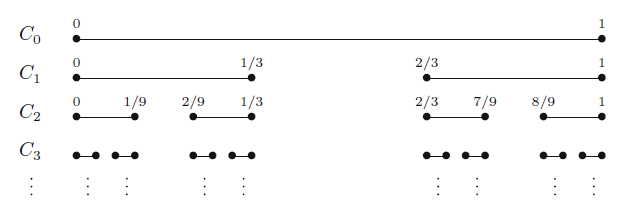
\includegraphics[width=\textwidth]{cantor-set}
  \caption{The Cantor set \cite{abbott2001understanding}}
  \label{fig:sup-inf}
\end{figure}

The question now is: what remains in $C$? 

Since $0 \in C_n$, for all $n \in \textbf{N}$, clearly $0 \in C$. By the same argument, $1 \in C$. And if $y$ is the endpoint of a closed interval in $C_n$, then $y$ is also an endpoint of one of the intervals of $C_{n+1}$. Hence, $y \in C_n$ for all $n \in \textbf{N}$, i.e., $y \in C$. Also notice that the endpoints are rational numbers of the form $m/3^n$.

It is reasonable that the length of $C$ is $1$ minus the total removed length:
\[
	\frac{1}{3} + 2 \left( \frac{1}{9} \right) + 4 \left( \frac{1}{27} \right) + \ldots + \left( 2^{n-1} \frac{1}{3^n} \right) + \ldots = \frac{1}{3} \sum \frac{2^{n-1}}{3^{n-1}} = \frac{1}{3} \frac{1}{1-\frac{2}{3}} = \frac{1}{3} 3 = 1
\]
Hence, the Cantor set has zero length.

We're going to show that $C$ is uncountable by constructing a bijection between $C$ and the set of sequences $(x_n)$, where $x_i \in \{0,1\}$ for all $i \in \textbf{N}$.

Let $x \in C$. Then, $x \in C_1$. We define
\begin{equation*}
  x_1 = \begin{cases}
      1, \text{ if $x$ is on the right side in $C_1$ } \\
  	  0, \text{ if $x$ is on the left side }
  \end{cases}
\end{equation*}

Repeating this process, we obtain a sequence of zeros and ones that corresponds to a point in the Cantor set. Since the set of sequences of zeros and ones is uncountable, then $C$ is also uncountable.

Another fact about the Cantor set is that $C$ has an empty interior.
\[
	\text{int} C = \{ p \in C : \exists \varepsilon > 0 \text{ such that } (p-\varepsilon, p+\varepsilon) \subseteq C \}
\]

To show that, let $p \in C$. Then given $\varepsilon > 0$, there exists $n_0 \in \textbf{N}$ such that $\frac{1}{3^{n_0}} < \varepsilon$. 

\begin{definition}[Perfect sets]
	A set $P \subseteq \textbf{R}$ is \textbf{perfect} if it is closed and doesn't contain isolated points, i.e., every point of $P$ is a limit point.
\end{definition}

\begin{example}
	Non-degenerated closed intervals $[a,b]$ are perfect.
\end{example}

In fact, the Cantor set is perfect. 

First, to show that $C$ is closed, remember that each $C_n$ is a finite union of closed intervals. Therefore, $C_n$ is closed. Since $C$ is an arbitrary intersection of closed sets, $C$ is closed.

Now, we need to show that $C$ contains no isolated point. Let $x \in C$. Let us construct a sequence $(x_n)$ of points of $C$, $x_n \neq x$ for all $n \in \textbf{N}$, and $x_n \to x$. Remember that the endpoints of each $C_n$ are contained in $C$.

Since $x \in C_1$, there exists $x_1 \in C_1 \cap C$ such that $x_1 \neq x$ and $|x - x_1| \leq \frac{1}{3}$. Analogously, for each $n \in \textbf{N}$, there exists $x_n \in C_n \cap C$, $x_n \neq x$, such that $|x - x_n| \leq 1/3^n$. Hence, $x_n \to x$.

\textbf{Exercise.} Show that a non-empty perfect set is uncountable.

\newpage

\section{Continuity}

In this section, our goal is to study the limit of a function and the concept of continuity.

\subsection{Functional Limit}

\begin{definition}[Functional Limit]
	Let $f : X \longrightarrow \textbf{R}$ be a real valued function defined on $X \subseteq \textbf{R}$, and let $a$ be a limit point of $X$. We say that $f$ goes to $L$ as $x$ goes to $a$, or simply
	\[
		\lim_{x \to a} f(x) = L
	\]
	if for every $\varepsilon > 0$, there exists a $\delta > 0$ such that whenever $0 < |x - a| < \delta$ it follows that
	\[
		|f(x) - L| < \varepsilon
	\]
\end{definition}

The definition of continuity can also be stated in terms of sequences.

\begin{theorem}
	Let $f : X \subseteq \textbf{R} \longrightarrow \textbf{R}$, and $a$ be a limit point of $X$. Then 
	\[
		\lim_{x \to a} f(x) = L \iff \lim_{n \to \infty} f(a_n) = L
	\]
	for every sequence $(a_n)$ in $X$ such that $a_n \neq a$ and $\lim_{n \to \infty} a_n = a$.
\end{theorem}

\begin{proof}
	Suppose that $\lim_{x \to a} f(x) = L$, and let $(a_n)$ be a sequence in $X$ such that $a_n \neq a$ and $\lim_{n \to \infty} a_n = a$.
	
	Given $\varepsilon > 0$, then there exists $\delta > 0$ such that $|f(x) - L| < \varepsilon$ if $x \in X$ and $0 < |x - a| < \delta$. Also, there exists $n_0 \in \textbf{N}$ such that $n > n_0$ implies $0 < |a_n - a| < \delta$. Therefore, for $n > n_0$, we have \[ | f(a_n) - L | < \varepsilon \] as desired.
	
	Now assume that $\lim_{x \to a} f(x) = L$ is false. Then, there exists $\varepsilon > 0$ such that for every $\delta > 0$ there exists a point $x \in X$, depending on $\delta$, for which $| f(x) - L | \geq \varepsilon$ but $0 < |x - a| < \delta$.
	
	Thus, taking $\delta_n = 1/n$, we find a sequence of points $a_n \in V_{\delta_n}(a)$, $(a_n) \to a$ and $a_n \neq a$ for all $n \in \textbf{N}$, where the sequence $f(a_n) \notin V_{\varepsilon}(L)$, i.e., $f(a_n)$ does not converge to $L$.
\end{proof}

\begin{corollary}
	If $f$ has a limit, then this limit is unique.
\end{corollary}

\begin{proof}
	Follows immediately from the theorem above and the fact that the limit of a sequence is unique.
\end{proof}

\begin{corollary}
	Let $f$ and $g$ be real valued functions defined on a domain $X \subseteq \textbf{R}$, and assume 
	\[
		\lim_{x \to a} f(x) = L \text{ and } \lim_{x \to a} g(x) = M
	\]
	for some limit point $a$ of $X$. Then,
	\begin{enumerate}
		\item $\lim_{x \to a} f(x) + g(x) = L + M$.
		\item $\lim_{x \to a} f(x) \cdot g(x) = LM$.
		\item $\lim_{x \to a} \frac{f(x)}{g(x)} = \frac{L}{M}$, if $M \neq 0$.
		\item $\lim_{x \to a} kf(x) = kL$ for all $k \in \textbf{R}$.
	\end{enumerate}
\end{corollary}

\begin{corollary}[Divergence Criterion for Functional Limits]
	Let $f : A \longrightarrow \textbf{R}$ and $a$ be a limit point of $X$. If there exists two sequences $(x_n)$ and $(y_n)$ in $X$ with $x_n \neq a$ and $y_n \neq a$ and
	\[
		\lim x_n = c = \lim y_n \text{ but } \lim f(x_n) \neq \lim f(y_n)
	\]
	then the limit $ \lim_{x \to a} f(x)$ does not exist.
\end{corollary}

\subsection{Continuous Functions}

The concept of continuity will help us avoid `unbroken curves' or functions with `jumps' and `holes'.

\begin{definition}[Continuity]
	A function $f : X \longrightarrow \textbf{R}$ is \textbf{continuous at a point} $c \in X$ if for every $\varepsilon > 0$, there exists $\delta > 0$ such that
	\[
		| f(x) - f(c) | < \varepsilon
	\]
	for all $x \in \textbf{R}$ for which $| x - c | < \delta$.
	
	If $f$ is continuous at every point of $X$, then $f$ is said to be \textbf{continuous on} $X$.
\end{definition}

One of the differences from this definition to the definition of functional limit is that we require $c$ to be in the domain of $f$.

An immediate result from this definition is that functions are continuous at isolated points of their domains.

And if $c$ is a limit point of $X$, then our definition of continuity can be rewritten as $\lim_{x \to c} f(x) = f(c)$.

\begin{example}
\begin{itemize} \hfill
	\item The constant function in $\textbf{R}$ is continuous.
	\item $f(x) = x$ is continuous at $\textbf{R}$.
\end{itemize}
\end{example}

\begin{theorem}
	Assume $f : I \longrightarrow \textbf{R}$ and $g : I \longrightarrow \textbf{R}$ are continuous at a point $c \in I$. Then,
	
	\begin{enumerate}
		\item $k f(x)$ is continuous at $c$ for all $k \in \textbf{R}$.
		\item $f(x) + g(x)$	is continuous at $c$.
		\item $f(x)g(x)$ is continuous at $c$.
		\item $f(x)/g(x)$ is continuous at $c$, provided that the quotient is defined.
	\end{enumerate}
\end{theorem}

\begin{proof}
	Let $(x_n) \in I$ such that $x_n \longrightarrow c$. Then we have $\lim f(x_n) = f(a)$ and $\lim g(x_n) = g(a)$. Then,
	\begin{equation*}
		\begin{aligned}
			\lim [f+g(x_n)] &= \lim [f(x_n) + g(x_n)] = \lim f(x_n) + \lim g(x_n) \\
			& = f(a) + g(a) = f+g(a)
		\end{aligned}
	\end{equation*}
	
	For the division,
	\begin{equation*}
		\begin{aligned}
			\lim \frac{f}{g} (x_n) &= \lim \frac{f(x_n)}{g(x_n)} = \frac{\lim f(x_n)}{\lim g(x_n)} \\
			&= \frac{f(a)}{g(a)} = \frac{f}{g} (a)
		\end{aligned}
	\end{equation*}
	
	And similarly for the product.
\end{proof}

This definition can be extended naturally for the whole interval $I$.

\begin{example}
\begin{itemize} \hfill
	\item $P(x) = a_n x^n + \ldots + a_1 x + a_0$ is continuous.
	\item If $p$ and $q$ are polynomials, then $p/q$ is continuous at the intervals in which $q \neq 0$.
\end{itemize}
\end{example}

\begin{theorem}[Composition of Continuous Functions]
	Let $f : A \longrightarrow \textbf{R}$ and $g : B \longrightarrow \textbf{R}$ be functions such that the range $f(A)$ is contained in the domain $B$, i.e., $f(A) \subseteq B$.
	
	If $f$ is continuous at $c \in A$, and $g$ is continuous at $f(c) \in B$, then the composition $g \circ f = g(f(x))$ is continuous at $c$.
\end{theorem}

\begin{proof}
	Consider a sequence $(x_n) \subseteq A$ such that $(x_n) \longrightarrow c$. Since $f$ is continuous at $c$, we have $f(x_n) \longrightarrow f(c)$. 
	
	Since $g$ is continuous at $f(c)$, we have $g(f(x_n)) \longrightarrow g(f(c))$.
	
	Hence, $g \circ f$ is continuous at $c$.
\end{proof}

\begin{theorem}
	A mapping $f : \textbf{R} \longrightarrow \textbf{R}$ is continuous if and only if the inverse image $f^{-1}(A)$ is open for every $A \subseteq \textbf{R}$.
\end{theorem}

\begin{proof}
	Suppose that $f$ is continuous on $\textbf{R}$ and $A \subseteq \textbf{R}$ be an open set. We will show that $f^{-1}(A)$ is an open set. 
	
	For each $a \in f^{-1}(A)$, we have $f(a) \in A$. Since $A$ is open, there exists $\varepsilon > 0$ such that $V_{\varepsilon}(f(a)) \subseteq A$. Since $f$ is continuous at $a$, for this $\varepsilon$ we associate a $\delta > 0$ such that
	\[
		f(V_{\delta}(a)) \subseteq V_{\varepsilon}(f(a)) \subseteq A
	\]
	Which means that $V_{\delta}(a) \subseteq f^{-1}(A)$ and, therefore, $f^{-1}(A)$ is open.
	
	Conversely, suppose that $f^{-1}(A)$ is open for every open set $A \subseteq \textbf{R}$. Let $\varepsilon > 0$, let $A' = V_{\varepsilon}(f(a))$ is open in $\textbf{R}$ and contains $f(a)$. By hypothesis, $A = f^{-1}(A')$ is open. Hence, there exists $\delta > 0$ such that
	\[
		V_{\delta}(a) \subseteq A \text{ and } f(V_{\delta}(a)) \subseteq V_{\varepsilon}(f(a))
	\]
	Therefore, $f$ is continuous.
\end{proof}

\begin{lemma}
	Let $f : I \longrightarrow \textbf{R}$ be a continuous function in $a \in I$. If $f(a) > 0$, then there exists $\delta > 0$ such that $f(x) > 0$ for all $x \in I \cap (a-\delta, a+ \delta)$.
\end{lemma}

\begin{proof}
	Since $f(a) > 0$, let $\varepsilon = f(a) / a$. Since $f$ is continuous at $a$, there exists $\delta > 0$ such that $|x-a| < \delta$ implies
	\begin{equation*}
		\begin{aligned}
			|f(x) - f(a)| < \varepsilon & \implies f(a) - \varepsilon < f(x) < f(a) + \varepsilon \\
			& \implies 0 < f(a) - \frac{f(a)}{2} < f(x) < f(a) + \frac{f(a)}{2}
		\end{aligned}
	\end{equation*}
	whenever $x \in I \cap V_{\delta}(a)$.
	
	And the proof is analogous for $f(a) < 0$.
\end{proof}

\begin{theorem}[Bolzano]\label{thm:bolzano-cont-fun}
	Let $f : [a,b] \longrightarrow \textbf{R}$ be a continuous function such that $f(a)f(b)<0$. Then there exists $c \in [a,b]$ such that $f(c) = 0$.
\end{theorem}

\begin{proof}
	Suppose, without loss of generality, that $f(a) < 0$ and $f(b) > 0$. We will consider the set \[ A = \{x \in [a,b] : f(x) < 0\} \]
	
	Since $A \subseteq [a,b]$, $A$ is bounded. And since $a \in A$, $A \neq \emptyset$. Let $c = \sup A$. We will show that $a < c$.
	
	And since $f(a) < 0$, there exists $\delta_1 > 0$ such that $a + \delta_1 < b$ and $f(x) < 0$ for all $x \in [a, a+\delta_1)$. hence, $c \geq a+\delta_1 > a$.
	
	Now we will show that $f(c) \leq 0$ and $c < b$. By the definition of supremum, there exists a sequence $(a_n) \subseteq A$ such that $a_n \longrightarrow c$. Since $f$ is continuous $f(a_n) \longrightarrow f(c)$. 
	
	Since $f(a_n) < 0$ for all $n \in \textbf{N}$, it follows that $f(c) \leq 0$. In particular, $c<b$ and, therefore, $a < c < b$.
	
	Suppose that $f(c) < 0$. Then there exists $\delta_2 > 0$ such that $(c - \delta_2, c+\delta_2) \subseteq [a,b]$ and $f(x) < 0$, for all $x \in (c - \delta_2, c+\delta_2)$.
	
	Hence, $V_{\delta_2}(c) \subseteq A$ and $c$ is not the supremum of $A$, which contradicts our hypothesis that $c = \sup A$. Hence, $f(c) = 0$.
\end{proof}

\begin{theorem}[Intermediate Value Theorem]
	Let $f:[a,b] \longrightarrow \textbf{R}$ be a continuous function. Then, for each $\gamma$ between $f(a)$ and $f(b)$, there exists $c \in [a,b]$ such that $f(c) = \gamma$.
\end{theorem}

\begin{proof}
	Suppose that $f(a) < \gamma < f(b)$. We define $g(x) = f(x) - \gamma$.
	
	Since $g$ is continuous, we have $g(a) = f(a) - \gamma < 0$. And $g(b) = f(b) \gamma > 0$.
	
	By the \hyperref[thm:bolzano-cont-fun]{Bolzano's theorem}, there exists $c \in (a,b)$ such that $g(c) = 0$, i.e., $f(c) - \gamma = 0$. Hence, $f(c) = \gamma$.
\end{proof}

\begin{definition}[Bounded functions]
	Let $f : I \subseteq \textbf{R} \longrightarrow \textbf{R}$.
	\begin{itemize}
		\item $f$ is \textbf{upper bounded} if there exists $B \in \textbf{R}$ such that $f(x) \leq B$, for all $x \in I$.
		\item $f$ is \textbf{lower bounded} if there exists $A \in \textbf{R}$ such that $A \leq f(x)$, for all $x \in I$.
		\item $f$ is \textbf{bounded} if $f$ is both upper bounded and lower bounded.
	\end{itemize}
\end{definition}

\begin{theorem}
	Every continuous functions $f : [a,b] \longrightarrow \textbf{R}$ is bounded.
\end{theorem}

\begin{proof}
	First, we are going to show that $f$ is upper bounded. Suppose that this is not the case. Then, there would be a sequence $(x_n) \subseteq [a,b]$ such that $f(x_n) > n$, for all $n \in \textbf{N}$.
	
	Since $[a,b]$ is compact, there exists a subsquence $(x_{n_k}) \subseteq (x_n)$ which converges to $x \in [a,b]$. And since $f$ is continuous, $f(x_{n_k})$ converges to $f(x)$. In particular, $f(x_{n_k})$ is bounded. But this contradicts our hypothesis that $f(x_{n_k}) > n_k$ for all $k \in \textbf{N}$.
	
	Analogously, we can proof that $f$ is lower bounded.
\end{proof}

\begin{theorem}[Weierstrass]
	Every continuous function $f : [a,b] \longrightarrow \textbf{R}$ has a maximum and minimum value, i.e., there exists $c, d \in [a,b]$ such that
	\[
		f(c) \leq f(x) \leq f(d) , \, \forall x \in [a,b]
	\]
\end{theorem}

\begin{proof}
	We already proved that $f$ is bounded, i.e., $f([a,b])$ is bounded. 
	
	Let $\beta = \sup \{ f([a,b]) \}$ and $\alpha = \inf \{ f([a,b]) \}$.
	
	By the definition of the supremum, there exists a sequence $(x_n) \subseteq [a,b]$ such that $f(x_n) \longrightarrow \beta$. Since $(x_n)$ is bounded, there exists a subsequence $(x_{n_k})$ which converges to a point $d \in [a,b]$.
	
	Now, since the function $f$ is continuous, we have $f(x_{n_k}) \longrightarrow f(d)$. Given that $f(x_{n_k})$ is a  subsequence of $f(x_n)$, we have $f(x_{n_k}) \longrightarrow \beta$, and hence $\beta = f(d) = \sup \{ f([a,b]) \}$.
	
	In an analogous way, it is proved that there exists $c \in [a,b]$ such that $f(c) = \alpha = \inf \{ f([a,b]) \}$. Therefore,
	\[
		f(c) \leq f(x) \leq f(d) , \, \forall x \in [a,b]
	\]
\end{proof}

\begin{example}
	$f:(0,1] \longrightarrow \textbf{R}$, where $f(x) = \frac{1}{x}$ does not have a maximum value.
\end{example}

The next theorem is an immediate consequence of the previous two theorems. However, we will present an alternative and elucidating proof.

\newpage

\begin{theorem}
	If $X \subseteq \textbf{R}$ is compact and $f$ is continuous, then $f(X)$ is compact.
\end{theorem}

\begin{proof}
	Suppose that $f : X \longrightarrow Y$ is a continuous function and $X$ is compact. 
	
	Let $\{ O_\lambda \}$ be an open cover of $f(X)$. Since $f$ is continuous, each set $f^{-1}(O_\lambda)$ is open. And since $X$ is compact, there are finitely many indices, $\lambda_1, \ldots, \lambda_n$, such that
	\[
		X \subseteq f^{-1}(O_{\lambda_1}) \cup \ldots \cup f^{-1}(O_{\lambda_n})
	\]
	
	Given the fact that $f(f^{-1}(X) \subseteq X$ for every $X \subseteq Y$, we have
	\[
		f(X) \subseteq O_{\lambda_1} \cup \ldots \cup O_{\lambda_n}
	\]
	which completes the proof.
\end{proof}

\subsection{Uniform Continuity}

Let $f : I \subseteq \textbf{R} \longrightarrow \textbf{R}$, and $x_o \in I$. Remember the definition of continuity. When does $\delta$ depends on $\delta (\varepsilon, x_0)$ and when does it only depends on $\varepsilon$? 

Consider the following example.

\begin{example}
	Let $f(x) = 3x+1$. We have that $f$ is continuous at $c \in \textbf{R}$.
	\[
		| f(x) - f(c) | = | 3x+1 - (3c+1) | = 3 |x-c|
	\]
	
	Hence, given $\varepsilon > 0$, choose $\delta = \varepsilon/3$.
	\[
		| x - c | < \delta \implies | f(x) - f(c) | = 3 |x-c| < 3 \frac{\varepsilon}{3} = \varepsilon
	\]
	
	And notice that $\delta$ only depends on $\varepsilon$.
\end{example}

\begin{example}
	Consider $f(x) = x^2$, which is continuous at $c \in \textbf{R}$. 
	\[
		| f(x) - f(c) | = |x^2 - c^2| = |(x-c)(x+c)| = |x-c| |x+c|
	\]
	
	It is necessary, in some way, to `control' the term $|x-c| |x+c|$. To do let, let $\varepsilon > 0$ be given.
	
	If we control $|x-c|$, we control the product. Suppose that $|x-c| < 1$. Then,
	\[
		|x+c| = |x-c + 2c| \leq |x-c| + |2c| < 1 + 2|c|
	\]
	
	If we also have $| x- c | < \frac{\varepsilon}{1 + 2 |c|}$, then
	\[
		|x-c| |x+c| < \frac{\varepsilon}{1+2|c|} (1+2|c|) = \varepsilon
	\]
	and $|f(x) - f(c)| < \varepsilon$.
	
	Taking $\delta = \min \left\{ 1, \frac{\varepsilon}{1+2|c|} \right\}$, given $x \in \textbf{R}$ we have that 
	\[
		|x-c| < \delta \implies |f(x) - f(c)| < \varepsilon
	\]
\end{example}

This examples motivate the succeeding definition.

\begin{definition}[Uniform continuity]
	Let $f : I \subseteq \textbf{R} \longrightarrow \textbf{R}$. We say that $f$ is \textbf{uniformly continuous} if for all $\varepsilon > 0$, there exists $\delta = \delta(\varepsilon) > 0$ such that if $x, y \in I$, and $|x-y| > \delta$, then $|f(x) - f(y)| < \varepsilon$.
\end{definition}

Please take notice on some of the differences between continuity and uniform continuity. Uniform continuity is defined on a set, whereas continuity can be defined at a single point.

The biggest difference is the fact that in uniform continuity, the $\delta$ in the definition depends only on $\varepsilon$, and not on any point $c$ in the interval. To say it in another way, if the function is uniformly continuous, we can find a single number $\delta > 0$ which will suffice to prove continuity for all points $c$ of the interval.

\begin{definition}[Lipschitz]
	Let $f : I \subseteq \textbf{R} \longrightarrow \textbf{R}$. We say that $f$ is \textbf{Lipschtiz} if there exists $M > 0$, such that 
	\[
		|f(x) - f(y) | \leq M |x-y| \, \forall x,y \in I
	\]
\end{definition}

\begin{example}
	\[
		| \sin(x) - \sin(y) | \leq |x-y|
	\]
\end{example}

\begin{theorem}
	Every Lipschitz function is uniformly continuous. 
\end{theorem}

\begin{proof}
	Let $f$ be a Lipschitz function. By definition, there exists $M > 0$ such that
	\[
		|f(x) - f(y) | \leq M |x-y| \, \forall x,y \in I
	\]
	
	Given $\varepsilon > 0$, let $\delta = \varepsilon/M$, which depends only on $\varepsilon$.
	
	If $|x-y| < \delta$, we have
	\[
		|f(x) - f(y) | \leq M |x-y| < M \delta = M \frac{\varepsilon}{M} = \varepsilon
	\]
\end{proof}

\begin{theorem}[Criterion for Discontinuity]
	Let $f : I \subseteq \textbf{R} \longrightarrow \textbf{R}$. Then $f$ is uniformly continuous if and only if for all pairs of sequences $(x_n)$ and $(y_n)$ in $I$ satisfying $x_n - y_n \longrightarrow 0$, we have that $f(x_n) - f(y_n) \longrightarrow 0$.
\end{theorem}

\begin{proof}
	$(\Rightarrow).$ Let $(x_n)$, $(y_n)$ be sequences in $I$ with $x_n - y_n \longrightarrow 0$. We are going to show that $f(x_n) - f(y_n) \longrightarrow 0$.
	
	Let $\varepsilon > 0$ be given. Since $f$ is uniformly continuous by hypothesis, there exists $\delta = \delta(\varepsilon) > 0$ such that
	\[
		|x_n - y_n| < \delta \implies |f(x_n) - f(y_n)| < \varepsilon
	\]
	
	Due to the fact that $x_n - y_n \longrightarrow 0$, there exists $n_0 \in \textbf{N}$ such that $|x_n - y_n| < \delta$ whenever $n > n_0$. Therefore, for all $n > n_0$, we have that 
	\[
		|f(x_n) - f(y_n)| < \varepsilon \text{ and } f(x_n) - f(y_n) \longrightarrow 0 
	\]
	
	$(\Leftarrow).$ Suppose that $f$ is not uniformly continuous. We are going to construct squences $(x_n)$ and $(y_n)$ in $I$ with $x_n - y_n \longleftarrow 0$ but $f(x_n) - f(y_n) \not\longrightarrow 0$.
	
	If $f$ does not satisfy the definition of uniform continuity, then there exists $\varepsilon > 0$ such that for all $\delta > 0$ there exists $x_\delta, \, y_\delta \in I$ with $| x_\delta - y_\delta | < \delta$ but $| f(x_\delta ) - f(y_\delta )| \geq \varepsilon$.
	
	Then, for $\varepsilon > 0$ (it exists!), we take $\delta = 1/n$, $n \in \textbf{N}$. In this way, we have $ |x_n - y_n| < 1/n$ and $x_n - y_n \longrightarrow 0$.
	
	Because of our hypothesis, we must have $f(x_n) - f(y_n) \longrightarrow 0$. However, $|f(x_n) - f(y_n)| \geq \varepsilon > 0$, for all $n \in \textbf{N}$, and $f(x_n) - f(y_n) \not\longrightarrow 0$, which is a contradiction.
\end{proof}

\begin{example}
	Show that $f : (0,1) \longrightarrow \textbf{R}$, $f(x) = 1/x$ is not uniformly continuous.
	
	Consider $x_n = \frac{1}{n}$ and $y_n = \frac{1}{2n}$. Then
	\[
		x_n - y_n = \frac{1}{n} - \frac{1}{2n} = \frac{1}{2n} \longrightarrow 0
	\]
	
	However,
	\[
		f(x_n) - f(y_n) = n - 2n = -n \not\longrightarrow 0
	\]
\end{example}

\begin{theorem}
	Let $K$ be a compact set. Then, every continuous function $f : K \longrightarrow \textbf{R}$ is uniformly continuous.
\end{theorem}

\begin{proof}
	Suppose that $f$ is not uniformly continuous. Then, there exists $\varepsilon > 0$ and $(x_n), (y_n) \subseteq [a,b]$ such that $x_n - y_n \longrightarrow $ and
	\[
		|f(x_n) - f(y_n)| \geq \varepsilon \, \forall n \in \textbf{N}
	\]
	
	Given that $(x_n) \subseteq [a,b]$ is a bounded sequence, $(x_n)$ has a convergent subsequence $(x_{n_k})_{k \in \textbf{N}}$, i.e., $x_{n_k} \longrightarrow x_0$ and $x_0 \in [a,b]$.
	
	Now, since $f$ is continuous at $x_0$, $f(x_{n_k}) \longrightarrow f(x_0)$.
	
	On the other hand, because $x_n - y_n \longrightarrow 0$, $x_{n_k} - y_{n_k} \longrightarrow 0$. Beyond that fact, since $x_{n_k} \longrightarrow x_0$, also $y_{n_k} \longrightarrow x_0$. Indeed, $y_{n_k} = x_{n_k} - (x_{n_k} - y_{n_k}) \longrightarrow x_0 - 0 = x_0$.
	
	Using the fact that $f$ is continuous at $x_0$, $f(y_{n_k}) \longrightarrow f(x_0)$. 
	
	Therefore,
	\[
		f(x_{n_k}) - f(y_{n_k}) \longrightarrow f(x_0) - f(x_0) == 0
	\]
	which contradicts our hypothesis that $|f(x_n) - f(y_n)| \geq \varepsilon$.
	
	Hence, $f$ is uniformly continuous.
\end{proof}

% R. 99, A. 129

\newpage
\nocite{*}
\bibliographystyle{alpha}
\bibliography{Analysis_Notes.bib}
\addcontentsline{toc}{section}{References}

%\appendix
%
%\newpage
%\section{Basic Topology: Elements of Set Theory}
%
%\subsection{Metric Spaces}
%
%Another useful tool in understanding real numbers is a very special function called \textbf{absolute value}.
%
%\begin{definition}[Absolute value]
%The \textbf{absolute value} of $x$, denoted by $|x|$ is defined as follows.
%	\[ | x | = 	
%	\begin{cases} 
%      x & \text{ if } x \geq 0 \\
%      -x & \text{ if } x < 0
%   \end{cases} \]
%\end{definition}
%
%\begin{theorem}
%	The absolute value function satisfies the following properties:
%	\begin{enumerate}
%		\item $|ab| = |a||b|$.
%		\item $|a+b| \leq |a| + |b|$ (\textbf{Triangle Inequality}).
%	\end{enumerate}
%\end{theorem}
%
%Notice that the absolute value $|b-a|$ is the \textbf{distance} between $a$ and $b$.
%
%With this notion, it is natural to name a space of points with a distance function, called metric. The name usually used for this is \textbf{`metric space'}.
%
%\begin{definition}
%	A set $X$, whose elements are called \textbf{points}, is said to be a \textbf{metric space} if for every two points $p, q \in X$ there is an associated real number $d(p,q)$, called the distance from $p$ to $q$ satisfying the following properties:
%	\begin{enumerate}
%		\item If $p \neq q$, then $d(p,q) > 0$. And $d(p,q) = 0$ iff. $p = q$.
%		\item $d(p,q) = d(q,p)$.
%		\item For any $r \in X$, $d(p,q) \leq d(p,r) + d(r,q)$.
%	\end{enumerate}
%\end{definition}
%
%\subsection{Euclidean Spaces}
%
%\begin{definition}[Vector Space]
%  For each positive integer $k$, let $\textbf{R}^k$ be the set of all ordered $k$-tuples $x = (x_1, x_2, \ldots, x_k)$ where $x_1, x_2, \ldots, x_k$ are real numbers, called the \textbf{coordinates} of $x$. The elements of $\textbf{R}^k$ are called points, or vectors. 
%
%  If $y = (y_1, y_2, \ldots, y_k)$ and $\alpha \in \textbf{R}$, we define addition of vectors and multiplication of a vector by a scalar as follows:
%  \[
%    x + y = (x_1 + y_1, \ldots, x_k + y_k)
%  \]
%  \[
%    \alpha x = (\alpha x_1, \ldots, \alpha x_k)
%  \]
%
%  These two operations satisfy the commutative, associative, and distributive laws. And $\textbf{R}^k$ is called a \textbf{vector space}.
%\end{definition}
%
%\begin{definition}[Inner Product]
%  Let $x, y \in \textbf{R}^k$. Then the \textbf{inner product} of $x$ and $y$ is defined by
%  \[
%    x \cdot y = \sum_{i=1}^k x_i y_i
%  \]
%\end{definition}
%
%\begin{definition}[Norm]
%  The \textbf{norm} of a vector $x$ is defined by
%  \[
%    | x | = \sqrt{(x \cdot x)}
%  \]
%\end{definition}
%
%\begin{definition}[Euclidean Space]
%  An \textbf{euclidean $k$-space} is a vector space $\textbf{R}^k$ with inner product and norm.
%\end{definition}
%
%\begin{theorem}
%  Let $x,y,z \in \textbf{R}^k$ and $\alpha$ be a scalar.
%  \begin{enumerate}
%    \item $|x| \geq 0$.
%    \item $|x| = 0$ iff. $x = 0$.
%    \item $|\alpha x| = |\alpha| |x|$.
%    \item $|x \cdot y| \leq |x| |y|$.
%    \item $|x + y| \leq |x| + |y|$.
%    \item $|x - z| \leq |x-y| + |y-z|$.
%  \end{enumerate}
%\end{theorem}
%
%\subsection{Finite, Countable, and Uncountable Sets}
%
%\begin{theorem}
%	Every infinite subset of a countable set is countable.
%\end{theorem}
%
%\begin{theorem}
%	Let $\{ E_n \}$, $n = 1, 2,3, \ldots$, be a sequence of countable sets, and put
%	\[
%		S = \bigcup_{n=1}^\infty E_n
%	\]
%	Then $S$ is countable.
%\end{theorem}
%
%\subsection{Metric Spaces}
%
%Intuitively, a metric space is a space of points with a distance function, called metric.
%
%\begin{definition} 
%	A set $X$, whose elements are called \textbf{points}, is said to be a \textbf{metric space} if for every two points $p, q \in X$ there is an associated real number $d(p,q)$, called the distance from $p$ to $q$ satisfying the following properties:
%	\begin{enumerate}
%		\item If $p \neq q$, then $d(p,q) > 0$. And $d(p,q) = 0$ iff. $p = q$.
%		\item $d(p,q) = d(q,p)$.
%		\item For any $r \in X$, $d(p,q) \leq d(p,r) + d(r,q)$.
%	\end{enumerate}
%\end{definition}
%
%\begin{example}
%	The Euclidean spaces $\textbf{R}^k$ are metric spaces with the distance function
%	\[
%		d(x,y) = | x - y |, \, (x,y \in \textbf{R}^k)
%	\]
%\end{example}
%
%Notice that if $Y$ is a subset of a metric space $X$, then $Y$ is also a metric space with the same distance function. Hence, every subset of an Euclidean space is a metric space.
%
%If $a_i < b_i$ for $i = 1, \ldots, k$, the set of all points $x = (x_1, \ldots, x_k) \in \textbf{R}^k$ whose coordinates satisfy the inequalities $a_i \leq x_i \leq b_i$, for $1 \leq i \leq k$, is called a \textbf{$k$-cell}.
%
%Examples: A $1$-cell is an interval, and a $2$-cell is a rectangle.
%
%\begin{definition}[Open and Closed Balls]
%	Let $x \in \textbf{R}^k$ and $r > 0$. The \textbf{open (resp. closed) ball} $B$ with center at $x$ and radius $r$ is defined as the set of all $y \in \textbf{R}^k$ such that $| y - x | < r$ (resp. $| y - x | \leq r$).
%\end{definition}
%
%\begin{definition}[Convex Sets]
%	A set $E \subseteq \textbf{R}^k$ is \textbf{convex} if
%	\[
%		\lambda x + (1-\lambda)y \in E
%	\]
%	whenever $x, y \in E$ and $0 < \lambda < 1$.
%\end{definition}
%
%\begin{definition}
%  Let $X$ be a metric space. All points and sets mentioned below are elements and subsets of $X$.
%  \begin{enumerate}
%    \item A \textbf{neighborhood} of a point $p$ is a set $N_r(p)$ consisting of all points $q$ such that $d(p,q) < r$. The number $r$ is called the \textbf{radius} of $N_r(p)$.
%    \item A point $p$ is a \textbf{limit point} of the set $E$ if every neighborhood of $p$ contains a point $q \neq p$ such that $q \in E$.
%    \item If $p \in E$ and $p$ is not a limit point of $E$, then $p$ is called an \textbf{isolated point} of $E$.
%    \item $E$ is \textbf{closed} if every limit point of $E$ is also a point of $E$.
%    \item A point $p$ is an \textbf{interior} point of $E$ if there is a neighborhood $N$ of $p$ such that $N \subseteq E$, i.e. every point of the neighborhood of $p$ is also inside $E$.
%    \item $E$ is \textbf{open} if every point of $E$ is an interior point. 
%    \item The \textbf{complement} of $E$, denoted by $E^c$, is the set of all points $p \in X$ such that $p \notin E$.
%    \item The set $E$ is called \textbf{perfect} if $E$ is closed and if every point of $E$ is a limit point of $E$.
%    \item $E$ is \textbf{bounded} if there is a real number $M$ and a point $q \in X$ such that $d(p,q) < M$ for all $p \in E$.
%    \item $E$ is \textbf{dense in $X$} if every point of $X$ is a limit point of $E$ or a point of $E$. 
%  \end{enumerate}  
%\end{definition}
%
%\begin{theorem}
%  Every neighbourhood is an open set.
%\end{theorem}
%
%\begin{theorem}
%  If $p$ is a limit point of a set $E$, then every neighbourhood of $p$ contains infinitely many points of $E$.
%\end{theorem}
%
%\begin{corollary}
%  A finite point set has no limit points.
%\end{corollary}
%
%\begin{theorem}
%  Let $\{ E_\alpha \}$ be a collection of sets. Then
%  \[
%    \left( \bigcup_{\alpha} E_\alpha \right)^c = \bigcap_{\alpha} \left( E_\alpha^c \right)
%  \]
%\end{theorem}
%
%\begin{theorem}
%  A set $E$ is open iff. its complement is closed. 
%\end{theorem}
%
%\begin{corollary}
%  A set is closed iff. its complement is open.
%\end{corollary}
%
%\begin{theorem} \hfill
%  \begin{enumerate}
%    \item For any collection $\{ G_\alpha \}$ of open sets, $\bigcup_{\alpha} G_{\alpha}$ is open.
%    \item For any collection $\{ F_\alpha \}$ of closed sets, $\bigcap_{\alpha} F_{\alpha}$ is closed.
%    \item For any finite collection $G_1, \ldots, G_n$ of open sets, $\bigcap_{i=1}^n G_i$ is open.
%    \item For any finite collection $F_1, \ldots, F_n$ of closed sets, $\bigcap_{i=1}^n F_i$ is closed.
%  \end{enumerate}
%\end{theorem}
%
%\begin{theorem}
%  Let $E$ be a closed set of real numbers which is bounded above. Let $y$ be the least upper bound of $E$. Then $y \in E$.
%\end{theorem}
%
%Define compact sets.
%
%\begin{theorem}
%	Compact subsets of metric spaces are closed.
%\end{theorem}
%
%\begin{theorem}
%	Closed subsets of compact sets are compact.
%\end{theorem}
%
%\begin{theorem}
%	Every $k$-cell is compact.
%\end{theorem}
%
%\begin{theorem}
%	Let $E \subseteq \textbf{R}^k$. The following properties are equivalent.
%	\begin{enumerate}
%		\item $E$ is closed and bounded.
%		\item $E$ is compact.
%		\item Every infinite subset of $E$ has a limit point in $E$.
%	\end{enumerate}
%\end{theorem}
%
%The equivalences $(1)$ and $(2)$ are known as the \textbf{Heine-Borel theorem}.
%
%\begin{theorem}[Weierstrass]
%	Every bounded infinite subset of $\textbf{R}^k$ has a limit point in $\textbf{R}^k$.
%\end{theorem}
%
%\begin{definition}[Connected Sets]
%	A set $E$ in a metric space $X$ is said to be \textbf{connected} if there do not exist two disjoint open subsets $A, B \subseteq X$ such that $A$ intersects $E$, $B$ intersects $E$, and $E \subseteq A \cup B$.
%	
%	In other words, let $X$ be a metric space. We say that $X$ is \textbf{disconnected} iff. there exist disjoint non-empty open sets $V, W$ in $X$ such that $V \cup W = X$, i.e., $X$ is disconnected iff. $X$ contains a non-empty proper subset which is closed and open. We say that $X$ is \textbf{connected} iff. it is non-empty and not disconnected. 
%\end{definition}
%
%\begin{theorem}
%	A subset $E$ of the real line $\textbf{R}$ is connected iff. whenever $x, y \in E$ and $x < z < y$, then $z \in E$.
%\end{theorem}
%
%\section{Numerical Sequences and Series}
%
%\subsection{Limits of sequences}
%
%\subsection{Cauchy Sequences}\label{cauchy-sequences}
%
%Goal: define real numbers as the limits of sequences of rational numbers.
%
%Which sequences of rational are convergent and which ones are not? 
%
%\begin{definition}[$\varepsilon$-steadiness]
%  A sequence $(a_n)_{n=m}^\infty$ is said \textbf{$\varepsilon$-steady} iff. each pair of sequence elements is $\varepsilon$-close, i.e., $|a_j - a_k| \leq \varepsilon$ for all $j,k \geq M$.
%
%  If there is an $N \geq 0$ such that $|a_j - a_k| \leq \varepsilon$ for $j, k \geq N$, then the sequence is said to be \textbf{eventually $\varepsilon$-steady}.
%\end{definition}
%
%\begin{definition}[Cauchy Sequences]
%  A sequence $(a_n)_{n=0}^\infty$ is said to be a \textbf{Cauchy sequence} iff. for every rational $\varepsilon > 0$, the sequence is eventually $\varepsilon$-steady. I.e., for every $\varepsilon > 0$, the exists an $N \geq 0$ such that $|a_j - a_k| \leq \varepsilon$ for $j, k \geq N$.
%\end{definition}
%
%\begin{definition}[Bounded Sequences]
%  A finite sequence is \textbf{bounded} by $M \geq 0$, $M \in \textbf{Q}$, iff. $|a_i| \leq M$ for all $1 \leq i \leq n$.   
%
%  An infinite sequence is \textbf{bounded} by $M$ iff. $|a_i| \leq M$ for all $i \geq 1$.
%\end{definition}
%
%\begin{lemma}
%  Every finite sequence $a_1, a_2, \ldots, a_n$ is bounded.
%\end{lemma}
%
%\begin{lemma}
%  Every Cauchy sequence $(a_n)_{n=1}^\infty$ is bounded.
%\end{lemma}
%
%\begin{proof}
%  Since $(a_n)_{n=1}^\infty$ is a Cauchy sequence, $a_n$ is an eventually $1$-steady and thus can be split into a finite sequence and a $1$-steady sequence, i.e., there is an $N \geq 0$ such that $|a_j - a_k| \leq 1$ for $j, k \geq N$.
%  
%  For the finite sequence, just apply the prior lemma, returning a boundary $M \geq 0$.
%
%  For the $1$-steady sequence, for all $j,k \geq N$ we have $|a_j - a_k| \leq 1$. Let $k = N$, $x = a_j - a_N$ and $y = a_N$. Then,
%  \[
%    | x + y | - | y | \leq |x| \iff |a_j| - |a_N| \leq |a_j - a_N| \leq 1
%  \]
%  
%  Hence,
%  \[
%    |a_j| \leq 1 + |a_N| \text{ for all } j \geq N
%  \]
%  which gives us the bound to the infinite tail of the sequence.
%
%  Finally, to find the bound over all the sequence, take $M' = M + 1 + |a_N|$. If $1 \leq n < N$, then $|a_n| \leq M \leq M'$. If $n \geq M$, then $|a_n| \leq 1 + |a_N| \leq M'$.
%\end{proof}

%Here $\lim$ is a formal limit. Later on we will define what exactly is a limit.
%
%\begin{lemma}[Sum of Cauchy sequences is Cauchy]
%  Let $x = \lim_{n \to \infty} a_n$ and $y = \lim_{n \to \infty} b_n$. Then $x+y$ is also a real number, i.e., $(a_n + b_n)_{n=1}^\infty$ is a Cauchy sequence of rationals.
%\end{lemma}
%
%The following lemma verifies the axiom of substitution:
%
%\begin{lemma}[Sum of equivalent Cauchy sequences are equivalent]
%  Let $x = \lim_{n \to \infty} a_n$, $y = \lim_{n \to \infty} b_n$, and $x' = \lim_{n \to \infty} a_n'$ be real numbers. Suppose that $x = x'$. Then we have $x+y = x'+y$.
%\end{lemma}
%
%\begin{proposition}[Multiplication is well defined]
%  Let $x = \lim_{n \to \infty} a_n$, $y = \lim_{n \to \infty} b_n$, and $x' = \lim_{n \to \infty} a_n'$ be real numbers. Then $xy$ is also a real number. If $x=x'$, then $xy = x'y$.
%\end{proposition}
%
%To define inverses/reciprocals, we need to restrict our Cauchy sequences from zero. To do this we use the following definition.
%
%\begin{definition}[Sequences bounded away from zero]
%  A sequence $(a_n)_{n=1}^\infty$ is said to be \textbf{bounded away from zero} iff. there exists a rational number $c > 0$ such that $|a_n| \geq c$ for all $n \geq 1$.
%\end{definition}
%
%\begin{definition}[Reciprocals of real numbers]
%  Let $x$ be a non-zero real number, $(a_n)_{n=1}^\infty$ a Cauchy sequence bounded away from zero such that $x = \lim_{n \to \infty} a_n$. Then we define the reciprocal $x^{-1}$ by the formula
%  \[
%    x^{-1} = \lim_{n \to \infty} a_n^{-1}
%  \]
%\end{definition}
%
%\begin{lemma}
%  Reciprocation is well defined.
%\end{lemma}
%
%Now our task is to order the real numbers. How can we define positive or negative reals? 
%
%\begin{definition}
%  Consider a sequence of rationals $(a_n)_{n=1}^\infty$. We say that this is sequence is \textbf{positively bounded away from zero} iff. there exists a rational $c > 0$ such that $a_n \geq c$ for all $n \geq 1$. A real number is said to be \textbf{positive} iff. it can be written as a Cauchy sequence that is positively bounded away from zero.
%
%  The sequence is \textbf{negatively bounded away from zero} iff. there exists a rational $-c < 0$ such that $a_n \leq -c$ for all $n \geq 1$. A real number is said to be \textbf{negative} iff. it can be written as a Cauchy sequence that is negatively bounded away from zero.
%\end{definition}
%
%\begin{definition}[Ordering of the real numbers]
%  Let $x$ and $y$ be real numbers. We say that $x$ is greater than $y$, and write $x > y$, if $x-y$ is a positive real number, and that $x$ is smaller than $y$, written $x < y$, if $x-y$ is a negative real number.
%\end{definition}

%\begin{proposition}[Bounding of reals by rationals]
%  Let $x$ be a positive real number. Then there exists a positive rational number $q$ such that $q \leq x$, and there exists a positive integer $N$ such that $x \leq N$.
%\end{proposition}
%
%\begin{corollary}[Archimedean property]
%  Let $x$ and $\varepsilon$ be any positive real numbers. Then there exists a positive integer $M$ such that $M \varepsilon > x$.
%
%  I.e. No matter how large $x$ is and how small $\varepsilon$ is, if one keeps adding $\varepsilon$ to itself, one will eventually overtake $x$.
%\end{corollary}
%
%\begin{proposition}
%  Given any two real numbers $x < y$, we can find a rational number $q$ such that $x < q < y$.
%\end{proposition}

%\subsection{The least upper bound property}
%
%\begin{definition}[Upper bound]
%  Let $E \subseteq \textbf{R}$, and let $M$ be a real number. We say that $M$ is an \textbf{upper bound} for $E$ iff. we have $x \leq M$ for every $x \in E$. Intuitivelly, an upper bound is a number that is greater or equal than every number in the given set.
%\end{definition}
%
%Since every larger number $M' \geq M$ is also an upper bound of $E$, but it is not always the case that a number smaller than $M$ is also an upper bound of $E$.
%
%\begin{definition}[Least upper bound]
%  Let $E \subseteq \textbf{R}$, and let $M$ be a real number. We say that $M$ is a \textbf{least upper bound} for $E$ iff. 
%  \begin{itemize}
%    \item $M$ is an upper bound for $E$.
%    \item Any other upper bound $M'$ for $E$ is larger than or equal to $M$.
%  \end{itemize}
%\end{definition}
%
%\begin{definition}[Supremum]
%  Let $E \subseteq \textbf{R}$. If $E$ is non-empty and has some upper bound, we define the \textbf{supremum of $E$} $\sup(E)$ to be the least upper bound of $E$. If $E$ is non-empty as has no upper bound, we set $\sup(E) := + \infty$. If $E$ is empty, we set $\sup(E) := - \infty$. 
%\end{definition}
%
%An example of how the least upper bound property is useful and that some numbers are real but not rational is the following
%
%\begin{proposition}
%  There exists a positive real number $x$ such that $x^2 = 2$.
%\end{proposition}
%
%Everything that we talked about upper bounds can also be applied for lower bounds, greatest lower bounds, and the infimum of a set.
%
%\begin{definition}
%  Let $x \geq 0$ be a non-negative real, and let $n \geq 1$ be a positive integer. We define $x^{1/n}$ by the formula
%  \[
%    x^{1/n} := \sup \{ y \in \textbf{R} : y \geq 0 \land y^n \leq x \}
%  \]
%\end{definition}
%
%\begin{lemma}[Existence of $n^\text{th}$ roots]
%  Let $x \geq 0$ be a non-negative real, and let $n \geq 1$ be a positive integer. Then the set $E := \{y \in \textbf{R} : y \geq 0 \land y^n \leq x \}$ is non-empty and is also bounded above. In particular, $x^{1/n}$ is a positive real number.
%\end{lemma}

\end{document}